\chapter{概率分布的比较}
\label{chap:distribution-comparison}

某个随机结果只取$0,1,2$三个值，关于它有两份概率表：
\[
 P=(0.6,\ 0.3,\ 0.1),\qquad Q=(0.3,\ 0.3,\ 0.4) .
\]
$P$是我们相信的规律，$Q$是另一个人给出的规律。两张表差多少？这个问题没有唯一的答案，答案取决于差别会在哪里造成后果。若关心的是某件事发生的概率，最坏的事件是“掷出$0$”，两边相差$0.3$。若用$Q$去预测按$P$产生的结果，要看的是$Q$在$P$常出现的地方给的概率是否太小，这牵涉到两表在同一点上的比值。若关心的是取值的平均，$P$下是$0.5$，$Q$下是$1.1$，相差$0.6$。若把取值看成直线上的位置，要把$P$的概率质量搬成$Q$的样子，搬动的质量乘以距离，总量至少是$0.6$。

再看一个更极端的例子。两个单点分布$\delta_0$与$\delta_h$，$h$是很小的正数。按事件看，它们完全不同：事件$\{0\}$在前者下概率为$1$，在后者下为$0$。按位置看，它们只差一个小平移。哪种看法对，取决于后续要用这个比较做什么：控制事件概率，控制似然比，控制某类函数的平均，还是控制位置的移动。

本章依次建立这四个角度的比较量。第一节用同一事件的概率差定义总变差，并把它写成密度差的积分和有界函数的期望差。第二节在同一参考测度下比较密度，得到KL散度、Hellinger距离、JS散度、$f$散度与Rényi散度，并证明随机后处理不会增大$f$散度。第三节用一类测试函数的期望差比较分布，核心是再生核Hilbert空间给出的核均值与MMD。第四节用耦合定义Wasserstein距离，并对一阶距离给出Lipschitz函数表示。

这四个角度互有交叉：总变差同时是事件比较、密度比较和有界函数比较，一阶Wasserstein距离同时是运输成本和Lipschitz函数比较。第五节固定一个评价函数，按它的有界性、Lipschitz性、RKHS范数或指数矩选用合适的比较量，给出期望误差的上界，并说明无界函数必须补充尾部条件。第六节研究一列分布的比较量趋于零能推出什么，把它们与第~\ref{chap:weak-convergence-of-distributions}章的弱收敛联系起来。

本章使用第~\ref{chap:probability-spaces}章的测度语言和Radon–Nikodym密度，第~\ref{chap:conditional-expectation}章的条件期望与条件Jensen不等式，以及第~\ref{chap:weak-convergence-of-distributions}章的弱收敛。分布由单个总体规律给出，本章不讨论怎样从样本估计这些量。

\section{总变差}
\label{sec:dcomp-tv}

最直接的比较是逐个事件对照：同一个事件$A$，在一个分布下概率是$P(A)$，在另一个分布下是$Q(A)$。只要所有事件的概率差都小，用$Q$代替$P$去回答“某事发生的概率是多少”就不会出大错。把所有事件中最坏的那个差拿出来，就得到一个数。本节先给出这个数的定义和计算方法，再把它从事件推广到有界函数的平均。

全章设$P,Q$是同一个可测空间$(\mathcal{X},\mathcal{F}_{\mathcal{X}})$上的概率测度。$\mathcal{X}$可以是有限集、$\mathbb{R}^{d}$或其他取值空间，事件指$\mathcal{F}_{\mathcal{X}}$中的集合。

\subsection{定义与计算}
\label{sec:dcomp-tv-definition}

把每个事件上的概率差取绝对值，再在全体事件上取上确界，就得到总变差。

\begin{definition}[总变差]
\label{def:dcomp-tv}
$P$与$Q$之间的\term{总变差}（total variation distance）是
\begin{equation}
 d_{\mathrm{TV}}(P,Q)=\sup_{A\in\mathcal{F}_{\mathcal{X}}}\bigl\lvert P(A)-Q(A)\bigr\rvert .
 \label{eq:dcomp-tv-def}
\end{equation}
\end{definition}

由定义可以直接读出几条性质。每个概率差都在$[-1,1]$中，所以$0\leq d_{\mathrm{TV}}\leq1$。交换$P,Q$不改变绝对值，所以它对称。对第三个分布$R$与任一事件$A$，
\[
 \lvert P(A)-R(A)\rvert\leq\lvert P(A)-Q(A)\rvert+\lvert Q(A)-R(A)\rvert ,
\]
两边取上确界得到三角不等式。$d_{\mathrm{TV}}(P,Q)=0$表示每个事件的概率都相同，即$P=Q$。所以总变差是全体概率测度上的一个距离。

\paragraph{有限概率表}
先在章首的例子上计算。$\mathcal{X}=\{0,1,2\}$，两份概率表是
\[
 p=(0.6,\ 0.3,\ 0.1),\qquad q=(0.3,\ 0.3,\ 0.4) .
\]
下文称它为\emph{例表}。三个点有$8$个子集，逐个计算$P(A)-Q(A)$，结果列在表~\ref{tab:dcomp-tv-events}中。差最大的是$\{0\}$与$\{0,1\}$，都等于$0.3$；最小的是$\{2\}$与$\{1,2\}$，都等于$-0.3$。所以$d_{\mathrm{TV}}(P,Q)=0.3$。

\begin{BookInlineTable}
 \centering
 \caption{例表中每个事件的概率差。}
 \label{tab:dcomp-tv-events}
 \begin{tabular}{lcccccccc}
  \toprule
  $A$ & $\varnothing$ & $\{0\}$ & $\{1\}$ & $\{2\}$ & $\{0,1\}$ & $\{0,2\}$ & $\{1,2\}$ & $\mathcal{X}$\\
  \midrule
  $P(A)-Q(A)$ & $0$ & $0.3$ & $0$ & $-0.3$ & $0.3$ & $0$ & $-0.3$ & $0$\\
  \bottomrule
 \end{tabular}
\end{BookInlineTable}

表中有规律可循。事件的概率差是各点概率差之和，点$0$贡献$+0.3$，点$1$贡献$0$，点$2$贡献$-0.3$。要让和最大，就把所有贡献为正的点放进事件，把贡献为负的点排除在外，见图~\ref{fig:dcomp-tv-table}。最坏事件是$\{x:p(x)>q(x)\}$，最大的差等于正的差之和。又因为两表各自总和为$1$，正的差之和等于负的差之和的绝对值，各占全部绝对差的一半：
\[
 d_{\mathrm{TV}}(P,Q)=\tfrac12\bigl(\lvert0.3\rvert+\lvert0\rvert+\lvert-0.3\rvert\bigr)=0.3 .
\]

\begin{BookInlineFigure}
 \centering
 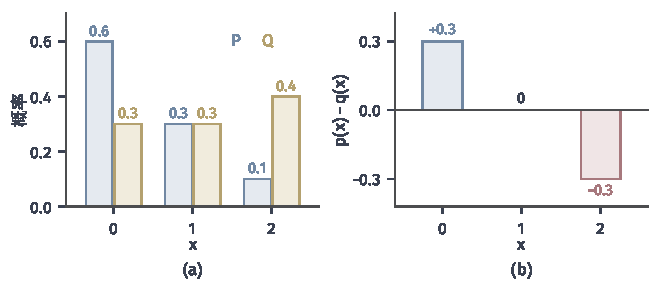
\includegraphics[width=112mm]{figures/07-probability/04-distribution-analysis/matplotlib/dcomp-tv-table/figure.pdf}
 \caption{例表的总变差。(a)蓝色柱为$P$，黄色柱为$Q$。(b)逐点概率差$p(x)-q(x)$，蓝色为正，红色为负。正的部分之和与负的部分之和的绝对值相等，都是$0.3$，即$d_{\mathrm{TV}}(P,Q)$。}
 \label{fig:dcomp-tv-table}
\end{BookInlineFigure}

\paragraph{共同支配测度}
要把这个规律推广到一般分布，需要一个能同时描述$P$与$Q$的“逐点概率”。有限表里它就是概率表本身；连续情形是密度；混有原子时两者都不够用。统一的办法是找一个测度$\lambda$，使$P,Q$都相对于它有密度。设$\lambda$是$\sigma$有限测度，并且$P\ll\lambda$，$Q\ll\lambda$，即$\lambda(A)=0$时$P(A)=Q(A)=0$。由Radon–Nikodym定理，存在非负可测函数$p,q$使
\begin{equation}
 P(A)=\int_{A}p\,\mathrm{d}\lambda,\qquad Q(A)=\int_{A}q\,\mathrm{d}\lambda,\qquad A\in\mathcal{F}_{\mathcal{X}},
 \label{eq:dcomp-common-density}
\end{equation}
并且$p,q$在$\lambda$几乎处处的意义下唯一，可参考\BookChapterRef{chap:measure-densities}{卷四第8章“测度的密度”}。这样的$\lambda$称为$P$与$Q$的\term{支配测度}（dominating measure），$p,q$称为它们相对于$\lambda$的密度。下文写$p,q$时，总是指相对于某个共同支配测度的密度。

支配测度总是存在：取$\lambda=P+Q$即可，因为$\lambda(A)=0$迫使$P(A)=Q(A)=0$。在有限表上$\lambda$取计数测度，$p,q$就是概率表；在$\mathbb{R}^{d}$上两者都有普通密度时，$\lambda$取Lebesgue测度。

\begin{theorem}[总变差的密度表示]
\label{thm:dcomp-tv-density}
设$p,q$是$P,Q$相对于共同支配测度$\lambda$的密度，$A^{*}=\{x:p(x)>q(x)\}$。则
\begin{equation}
 d_{\mathrm{TV}}(P,Q)=\frac12\int\lvert p-q\rvert\,\mathrm{d}\lambda=P(A^{*})-Q(A^{*})=1-\int\min(p,q)\,\mathrm{d}\lambda .
 \label{eq:dcomp-tv-density}
\end{equation}
\end{theorem}

\begin{proof}
先说明$A^{*}$达到上确界。对任一事件$A$，把它拆成$A\cap A^{*}$与$A\setminus A^{*}$。在$A^{*}$上$p-q>0$，在其外$p-q\leq0$，所以
\[
 P(A)-Q(A)=\int_{A}(p-q)\,\mathrm{d}\lambda\leq\int_{A\cap A^{*}}(p-q)\,\mathrm{d}\lambda\leq\int_{A^{*}}(p-q)\,\mathrm{d}\lambda .
\]
第一步丢掉了非正的部分，第二步补上了非负的部分。右端就是$P(A^{*})-Q(A^{*})$。同理，$Q(A)-P(A)\leq Q(B)-P(B)$，其中$B=(A^{*})^{\mathrm{c}}$。

再说明两个方向的最大值相等。两个密度的积分都是$1$，所以$\int(p-q)\,\mathrm{d}\lambda=0$，把积分拆到$A^{*}$与$B$上，得到
\[
 \int_{A^{*}}(p-q)\,\mathrm{d}\lambda=\int_{B}(q-p)\,\mathrm{d}\lambda .
\]
因此$\lvert P(A)-Q(A)\rvert$的上确界等于$P(A^{*})-Q(A^{*})$，即式~\eqref{eq:dcomp-tv-density}的第二个表达式。

$\lvert p-q\rvert$在$A^{*}$上等于$p-q$，在$B$上等于$q-p$。由上式，两部分积分相等，所以$\int\lvert p-q\rvert\,\mathrm{d}\lambda$是它们的两倍，这给出第一个表达式。最后，由$\lvert p-q\rvert=p+q-2\min(p,q)$，
\[
 \frac12\int\lvert p-q\rvert\,\mathrm{d}\lambda=\frac12\Bigl(1+1-2\int\min(p,q)\,\mathrm{d}\lambda\Bigr)=1-\int\min(p,q)\,\mathrm{d}\lambda .
\]
\end{proof}

式~\eqref{eq:dcomp-tv-density}的左端按定义~\eqref{eq:dcomp-tv-def}计算，与$\lambda$无关，所以右端也与支配测度的选取无关。最后一个表达式给出一个面积图景：$\int\min(p,q)\,\mathrm{d}\lambda$是两个密度的重叠部分，总变差是$1$减去重叠，也就是一个分布中“没有被另一个分布覆盖”的质量。

\paragraph{两个高斯分布}
取$P=\mathcal{N}(0,1)$，$Q=\mathcal{N}(1,1)$，以Lebesgue测度为支配测度。两个密度在$x=1/2$处相等，左侧$p>q$，所以$A^{*}=(-\infty,1/2)$。由式~\eqref{eq:dcomp-tv-density}，
\[
 d_{\mathrm{TV}}(P,Q)=\Phi\Bigl(\frac12\Bigr)-\Phi\Bigl(\frac12-1\Bigr)=2\Phi\Bigl(\frac12\Bigr)-1\approx0.3829 .
\]
图~\ref{fig:dcomp-tv-gaussians}(a)中浅蓝区域的面积是$\int(p-q)^{+}\,\mathrm{d}x$，浅黄区域是$\int(q-p)^{+}\,\mathrm{d}x$，两块面积相等，都是总变差。

\paragraph{没有共同普通密度的情形}
取
\[
 P=\operatorname{Unif}(0,1),\qquad Q=\tfrac12\operatorname{Unif}(0,1)+\tfrac12\delta_{1/2},
\]
即$Q$以一半概率均匀取值，另一半概率恰好取$1/2$。$Q$在单点$1/2$上有正概率，它没有Lebesgue密度。取$\lambda$为$(0,1)$上的Lebesgue测度加上$1/2$处的单位点质量，两个分布都被它支配，密度是
\[
 p(x)=\begin{cases}1,&x\in(0,1)\setminus\{\tfrac12\},\\0,&x=\tfrac12,\end{cases}\qquad
 q(x)=\begin{cases}\tfrac12,&x\in(0,1)\setminus\{\tfrac12\},\\\tfrac12,&x=\tfrac12 .\end{cases}
\]
在$x=1/2$处，$p$取$0$是因为$P(\{1/2\})=0$，而这一点上$\lambda$的质量是$1$，$q$必须等于$Q(\{1/2\})=1/2$。由式~\eqref{eq:dcomp-tv-density}，
\[
 d_{\mathrm{TV}}(P,Q)=\frac12\Bigl(\int_0^1\Bigl\lvert1-\frac12\Bigr\rvert\,\mathrm{d}x+\Bigl\lvert0-\frac12\Bigr\rvert\Bigr)=\frac12 .
\]
直接用定义检验：事件$\{1/2\}$的概率差就是$1/2$。图~\ref{fig:dcomp-tv-gaussians}(b)把原子画成竖线，它相对于$\lambda$的“密度”是该点的概率。

\begin{BookInlineFigure}
 \centering
 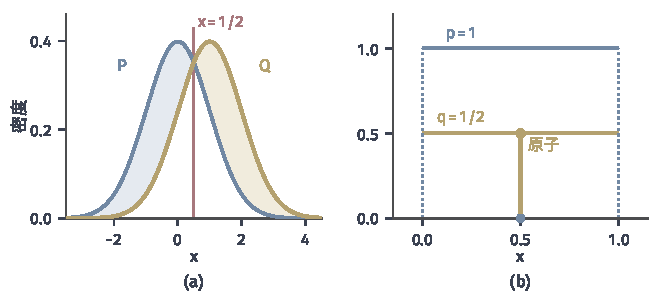
\includegraphics[width=112mm]{figures/07-probability/04-distribution-analysis/matplotlib/dcomp-tv-gaussians/figure.pdf}
 \caption{总变差的计算。(a)$P=\mathcal{N}(0,1)$（蓝）与$Q=\mathcal{N}(1,1)$（黄），红线是$x=1/2$；浅蓝区域$\{p>q\}$与浅黄区域$\{q>p\}$的面积都等于$d_{\mathrm{TV}}(P,Q)\approx0.3829$。(b)$P=\operatorname{Unif}(0,1)$（蓝）与$Q=\tfrac12\operatorname{Unif}(0,1)+\tfrac12\delta_{1/2}$（黄）相对于“Lebesgue测度加$1/2$处点质量”的密度；黄色竖线是$Q$在$1/2$处的原子，蓝点表示$P$在该点的密度为$0$。}
 \label{fig:dcomp-tv-gaussians}
\end{BookInlineFigure}

\paragraph{总变差看不到距离}
单点分布$\delta_x$与$\delta_y$（$x\neq y$）的总变差总是$1$：事件$\{x\}$在前者下概率为$1$，在后者下为$0$。无论$x,y$相距多近，结果都一样。更一般地，若存在事件$A$使$P(A)=1$，$Q(A)=0$，即$P$与$Q$相互奇异，则$d_{\mathrm{TV}}(P,Q)=1$，取到最大值。总变差只问“同一个事件的概率是否相同”，不问取值之间有多远。第~\ref{sec:dcomp-wasserstein}节会用位置移动的成本补上这个缺口。

\subsection{有界函数的期望差}
\label{sec:dcomp-tv-functions}

事件的概率是示性函数的期望：$P(A)=\mathbb{E}_{P}[\mathbf{1}_{A}]$。若关心的不是某件事是否发生，而是一个有界的数值结果，例如有上限的损失，那么要比较的是$\mathbb{E}_{P}[g]$与$\mathbb{E}_{Q}[g]$。总变差同样能控制它们，只是系数取决于$g$的取值范围。

\begin{theorem}[有界函数的期望差]
\label{thm:dcomp-tv-bounded}
设$g:\mathcal{X}\to\mathbb{R}$可测且有界，记$\operatorname{osc}(g)=\sup g-\inf g$。则
\begin{equation}
 \bigl\lvert\mathbb{E}_{P}[g]-\mathbb{E}_{Q}[g]\bigr\rvert\leq\operatorname{osc}(g)\,d_{\mathrm{TV}}(P,Q)\leq2\lVert g\rVert_{\infty}\,d_{\mathrm{TV}}(P,Q),
 \label{eq:dcomp-tv-osc}
\end{equation}
其中$\lVert g\rVert_{\infty}=\sup\lvert g\rvert$。并且
\begin{equation}
 \sup_{\lVert g\rVert_{\infty}\leq1}\bigl\lvert\mathbb{E}_{P}[g]-\mathbb{E}_{Q}[g]\bigr\rvert=2\,d_{\mathrm{TV}}(P,Q),
 \label{eq:dcomp-tv-dual}
\end{equation}
上确界在$g^{\pm}$处达到，$g^{\pm}$在$A^{*}$上取$1$，在其外取$-1$。
\end{theorem}

\begin{proof}
用共同支配测度写出期望差$\int g\,(p-q)\,\mathrm{d}\lambda$。因为$\int(p-q)\,\mathrm{d}\lambda=0$，被积函数中的$g$可以减去任意常数$c$而不改变积分：
\[
 \mathbb{E}_{P}[g]-\mathbb{E}_{Q}[g]=\int\bigl(g-c\bigr)(p-q)\,\mathrm{d}\lambda .
\]
取$c=(\sup g+\inf g)/2$，则$\lvert g-c\rvert\leq\operatorname{osc}(g)/2$处处成立。于是
\[
 \bigl\lvert\mathbb{E}_{P}[g]-\mathbb{E}_{Q}[g]\bigr\rvert\leq\frac{\operatorname{osc}(g)}{2}\int\lvert p-q\rvert\,\mathrm{d}\lambda=\operatorname{osc}(g)\,d_{\mathrm{TV}}(P,Q),
\]
最后一步用了式~\eqref{eq:dcomp-tv-density}。又$\operatorname{osc}(g)\leq2\lVert g\rVert_{\infty}$，得到式~\eqref{eq:dcomp-tv-osc}。

对$\lVert g\rVert_{\infty}\leq1$，上式给出期望差不超过$2d_{\mathrm{TV}}$。取$g=g^{\pm}$，则$g(p-q)=\lvert p-q\rvert$，期望差恰好是$\int\lvert p-q\rvert\,\mathrm{d}\lambda$，即$2d_{\mathrm{TV}}$，所以式~\eqref{eq:dcomp-tv-dual}的上确界达到。
\end{proof}

减去常数这一步是关键。概率差只对“质量怎样重新分配”敏感，整体平移$g$不影响结果，所以真正起作用的是$g$的振幅$\operatorname{osc}(g)$，而不是它的绝对大小。

\paragraph{系数的两种约定}
定义~\eqref{eq:dcomp-tv-def}在事件上取上确界，等价于在取值于$[0,1]$的函数上取上确界：这样的$g$满足$\operatorname{osc}(g)\leq1$，由式~\eqref{eq:dcomp-tv-osc}，期望差不超过$d_{\mathrm{TV}}$，而示性函数$\mathbf{1}_{A^{*}}$达到它。若改在单位球$\lVert g\rVert_{\infty}\leq1$上取上确界，函数可以从$-1$变到$1$，振幅加倍，结果是$2d_{\mathrm{TV}}$。有些文献把$\int\lvert p-q\rvert\,\mathrm{d}\lambda$称为总变差，它是本书$d_{\mathrm{TV}}$的两倍。读到“总变差小于$\varepsilon$”时，要先确认用的是哪一种约定。

\paragraph{例表上的检验}
在例表上取$g=g^{\pm}$。这里$A^{*}=\{0\}$，$g$在三个点上依次取$1,-1,-1$，两个期望是
\[
 \mathbb{E}_{P}[g]=0.6-0.3-0.1=0.2,\qquad\mathbb{E}_{Q}[g]=0.3-0.3-0.4=-0.4 .
\]
差为$0.6$，正是$2d_{\mathrm{TV}}$。再取$g(x)=x$，它的振幅是$2$，式~\eqref{eq:dcomp-tv-osc}给出的上界与实际的差分别是
\[
 2\times0.3=0.6,\qquad\lvert0.5-1.1\rvert=0.6,
\]
上界恰好达到。原因是$x=1-\tilde{g}(x)$，其中$\tilde{g}$在三点上依次取$1,0,-1$，而$\tilde{g}$正好在$p>q$处取最大值、在$p<q$处取最小值。一般的有界函数没有这样的巧合，上界会有余量。

式~\eqref{eq:dcomp-tv-dual}把总变差写成一类测试函数上的最大期望差。第~\ref{sec:dcomp-ipm}节会换用别的函数类得到别的比较量，第~\ref{sec:dcomp-expectation}节会把这个结果与其他比较量的类似结果放在一起，按评价函数的性质选择。

\section{密度比较}
\label{sec:dcomp-density}

总变差只用到密度之差$\lvert p-q\rvert$。看两个位置：一处$p=0.02$，$q=0.01$；另一处$p=0.51$，$q=0.50$。两处的差都是$0.01$，对总变差的贡献相同。可是若用$Q$去预测按$P$产生的结果，第一处的结果实际出现的频率是$Q$所说的两倍，第二处只多了百分之二。比值$p(x)/q(x)$记录的正是这种相对失衡。

本节在同一个支配测度$\lambda$下比较同一位置上的两个密度，用对数比、平方根和幂次构造几种比较量，再把它们归入同一个机制：对密度比施加一个凸函数，再求平均。密度为零的位置需要单独约定，而且多数比较量不对称或不满足三角不等式，所以统称为散度，只有满足距离公理的才称为距离。

\subsection{KL散度}
\label{sec:dcomp-kl}

\paragraph{对数比的平均}
设观测到一个结果$x$，要判断它更像来自$P$还是$Q$。比值$p(x)/q(x)$大于$1$时支持$P$，取对数后$\ln(p(x)/q(x))$大于零。对数的好处是独立观测的证据可以相加：$n$次独立观测的密度比是各次比值的乘积，取对数就成了各次对数比之和。如果数据确实来自$P$，每次观测平均提供的证据是对数比在$P$下的期望。由第~\ref{chap:laws-of-large-numbers}章的强大数律，只要这个期望存在，$n$次观测的总证据除以$n$几乎必然趋于它，所以它衡量的是“$P$为真时，平均每次观测能把$P$与$Q$分开多少”。

对数比在$q(x)=0<p(x)$处是$+\infty$：$P$下可能出现、$Q$却认为不可能的结果，一旦出现就彻底否定$Q$。在$p(x)=0$处，这个点在$P$下不出现，对平均没有贡献。定义据此处理零密度。

\begin{definition}[KL散度]
\label{def:dcomp-kl}
设$p,q$是$P,Q$相对于共同支配测度$\lambda$的密度。若$P\ll Q$，定义$P$相对于$Q$的\term{KL散度}（Kullback--Leibler divergence）为
\begin{equation}
 D_{\mathrm{KL}}(P\Vert Q)=\int_{\{p>0\}}p\ln\frac{p}{q}\,\mathrm{d}\lambda=\mathbb{E}_{P}\Bigl[\ln\frac{\mathrm{d}P}{\mathrm{d}Q}\Bigr] ;
 \label{eq:dcomp-kl-def}
\end{equation}
若$P$不绝对连续于$Q$，定义$D_{\mathrm{KL}}(P\Vert Q)=+\infty$。
\end{definition}

定义里有两件事需要核对。第一，积分有意义。$P\ll Q$时$P(q=0)=0$，被积函数在$\{p>0\}$上$\lambda$几乎处处有限。它的负部只出现在$p<q$处，由$\ln u\leq u-1$，
\[
 \int_{\{0<p<q\}}p\ln\frac{q}{p}\,\mathrm{d}\lambda\leq\int_{\{0<p<q\}}p\Bigl(\frac{q}{p}-1\Bigr)\,\mathrm{d}\lambda\leq\int q\,\mathrm{d}\lambda=1 .
\]
负部的积分有限，所以整个积分在$(-\infty,+\infty]$中有确定的值。第二，结果与$\lambda$无关：$P\ll Q$时比值$p/q$在$P$几乎处处的意义下就是Radon–Nikodym密度$\mathrm{d}P/\mathrm{d}Q$，式~\eqref{eq:dcomp-kl-def}的最后一个表达式里没有$\lambda$。

\begin{theorem}[Gibbs不等式]
\label{thm:dcomp-gibbs}
$D_{\mathrm{KL}}(P\Vert Q)\geq0$，等号成立当且仅当$P=Q$。
\end{theorem}

\begin{proof}
若$P$不绝对连续于$Q$，散度为$+\infty$，结论成立。设$P\ll Q$。在$\{p>0\}$上用$\ln u\leq u-1$（等号仅在$u=1$时成立），取$u=q/p$，
\[
 -D_{\mathrm{KL}}(P\Vert Q)=\int_{\{p>0\}}p\ln\frac{q}{p}\,\mathrm{d}\lambda\leq\int_{\{p>0\}}(q-p)\,\mathrm{d}\lambda=Q(p>0)-1\leq0 .
\]
若等号成立，第一个不等号要求$\lambda$几乎处处在$\{p>0\}$上$q=p$，第二个要求$Q(p>0)=1$，即$Q$在$\{p=0\}$上没有质量。两条合起来就是$p=q$几乎处处，即$P=Q$。
\end{proof}

这个结论称为\term{Gibbs不等式}（Gibbs' inequality）。证明里用的$\ln u\leq u-1$是对数函数位于它在$u=1$处切线下方，即凹性。KL散度非负，是因为在$P$自己的权重下，“用$Q$的概率”平均起来不如“用$P$自己的概率”。

\paragraph{方向不对称}
在例表上逐项计算。点$1$处$p=q$，贡献为零；另外两项是
\[
 0.6\ln\frac{0.6}{0.3}=0.6\ln2,\qquad 0.1\ln\frac{0.1}{0.4}=-0.2\ln2 .
\]
两项相加，
\[
 D_{\mathrm{KL}}(P\Vert Q)=0.4\ln2\approx0.2773 .
\]
交换两表，同样的两个位置贡献$0.3\ln(1/2)=-0.3\ln2$与$0.4\ln4=0.8\ln2$，
\[
 D_{\mathrm{KL}}(Q\Vert P)=0.5\ln2\approx0.3466 .
\]
两个方向的数值不同。单项可以为负（例如点$2$处$p<q$），总和却不为负，这正是Gibbs不等式。图~\ref{fig:dcomp-kl-asymmetry}(a)画出各项的贡献：$D_{\mathrm{KL}}(Q\Vert P)$的大头来自点$2$，那里$Q$有$0.4$的质量而$P$只给$0.1$。

\paragraph{高斯分布}
取$P=\mathcal{N}(\mu_1,\sigma_1^{2})$，$Q=\mathcal{N}(\mu_2,\sigma_2^{2})$。两个密度之比的对数是
\[
 \ln\frac{p(x)}{q(x)}=\ln\frac{\sigma_2}{\sigma_1}-\frac{(x-\mu_1)^{2}}{2\sigma_1^{2}}+\frac{(x-\mu_2)^{2}}{2\sigma_2^{2}} .
\]
在$P$下取期望，$\mathbb{E}_{P}[(X-\mu_1)^{2}]=\sigma_1^{2}$，而
\[
 \mathbb{E}_{P}\bigl[(X-\mu_2)^{2}\bigr]=\sigma_1^{2}+(\mu_1-\mu_2)^{2} .
\]
代入得到
\begin{equation}
 D_{\mathrm{KL}}(P\Vert Q)=\ln\frac{\sigma_2}{\sigma_1}+\frac{\sigma_1^{2}+(\mu_1-\mu_2)^{2}}{2\sigma_2^{2}}-\frac12 .
 \label{eq:dcomp-kl-gauss}
\end{equation}
方差相同时它化为$(\mu_1-\mu_2)^{2}/(2\sigma^{2})$，两个方向相等。尺度不同时不对称。图~\ref{fig:dcomp-kl-asymmetry}(b)固定$P=\mathcal{N}(0,1)$，令$Q_s=\mathcal{N}(0,s^{2})$。$s<1$时$Q_s$比$P$窄，$P$在两侧尾部的质量落在$Q_s$密度极小的地方，$D_{\mathrm{KL}}(P\Vert Q_s)$迅速增大；反过来，$D_{\mathrm{KL}}(Q_s\Vert P)$在$s<1$时保持较小。KL散度惩罚的是：参考分布$Q$在$P$有质量的地方给出太小的概率。

\begin{BookInlineFigure}
 \centering
 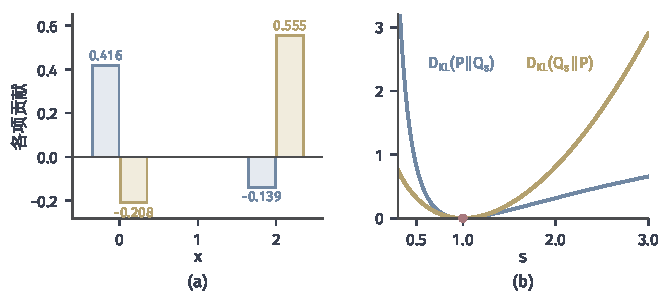
\includegraphics[width=112mm]{figures/07-probability/04-distribution-analysis/matplotlib/dcomp-kl-asymmetry/figure.pdf}
 \caption{KL散度的方向。(a)例表中各点的贡献：蓝色为$p\ln(p/q)$，合计$0.4\ln2\approx0.2773$；黄色为$q\ln(q/p)$，合计$0.5\ln2\approx0.3466$。(b)$P=\mathcal{N}(0,1)$，$Q_s=\mathcal{N}(0,s^{2})$，蓝线为$D_{\mathrm{KL}}(P\Vert Q_s)$，黄线为$D_{\mathrm{KL}}(Q_s\Vert P)$，红点是$s=1$。}
 \label{fig:dcomp-kl-asymmetry}
\end{BookInlineFigure}

\paragraph{绝对连续不保证有限}
$P\ll Q$只排除了“$Q$认为不可能、$P$却可能”的事件，并不保证对数比的平均有限。取$P$为标准Cauchy分布，$Q=\mathcal{N}(0,1)$。两个密度处处为正，互相绝对连续。对数比为
\[
 \ln\frac{p(x)}{q(x)}=\frac{x^{2}}{2}-\ln\bigl(1+x^{2}\bigr)+\ln\sqrt{\frac{2}{\pi}} .
\]
当$\lvert x\rvert$足够大时，右边不小于$x^{2}/4$，而Cauchy分布下$\mathbb{E}_{P}[X^{2}]=+\infty$，所以$D_{\mathrm{KL}}(P\Vert Q)=+\infty$。反方向的散度是对数比的相反数在$\mathcal{N}(0,1)$下的期望，其中$X^{2}$与$\ln(1+X^{2})$都可积，所以$D_{\mathrm{KL}}(Q\Vert P)$有限。用尾部很轻的高斯分布去预测重尾的Cauchy结果，代价是无穷大；反过来则不然。

\subsection{Hellinger距离}
\label{sec:dcomp-hellinger}

KL散度不对称，可以是无穷大，并且对零密度极为敏感。若想要一个真正的距离，可以先把密度开平方。$\sqrt{p}$满足$\int(\sqrt{p})^{2}\,\mathrm{d}\lambda=1$，即它是$L^{2}(\lambda)$中的单位向量。于是每个分布对应单位球面上的一个点，两个分布之间可以用这两个点的欧氏距离比较。

\begin{definition}[Hellinger距离与Bhattacharyya系数]
\label{def:dcomp-hellinger}
设$p,q$是$P,Q$相对于共同支配测度$\lambda$的密度。称
\begin{equation}
 d_{\mathrm{H}}(P,Q)=\frac{1}{\sqrt2}\bigl\lVert\sqrt{p}-\sqrt{q}\bigr\rVert_{L^{2}(\lambda)}=\Bigl(\frac12\int\bigl(\sqrt{p}-\sqrt{q}\bigr)^{2}\,\mathrm{d}\lambda\Bigr)^{1/2}
 \label{eq:dcomp-hellinger-def}
\end{equation}
为\term{Hellinger距离}（Hellinger distance），称
\begin{equation}
 B(P,Q)=\int\sqrt{pq}\,\mathrm{d}\lambda
 \label{eq:dcomp-bhattacharyya-coefficient}
\end{equation}
为\term{Bhattacharyya系数}（Bhattacharyya coefficient）。
\end{definition}

把式~\eqref{eq:dcomp-hellinger-def}中的平方展开，两个密度的积分都是$1$，交叉项正是$B$：
\begin{equation}
 d_{\mathrm{H}}^{2}(P,Q)=\frac12\int\bigl(p+q-2\sqrt{pq}\bigr)\,\mathrm{d}\lambda=1-B(P,Q) .
 \label{eq:dcomp-hellinger-bc}
\end{equation}
由Cauchy--Schwarz不等式，$B$不超过$\sqrt{p}$与$\sqrt{q}$的$L^{2}$范数之积，即$1$；又$B\geq0$，所以$0\leq d_{\mathrm{H}}\leq1$。$d_{\mathrm{H}}=1$当且仅当$B=0$，即$pq=0$几乎处处，两个分布相互奇异。系数$1/\sqrt2$正是为了让最大值等于$1$。$d_{\mathrm{H}}$是$L^{2}(\lambda)$中两个向量之差的范数乘以常数，所以对称并满足三角不等式；$d_{\mathrm{H}}=0$表示$\sqrt{p}=\sqrt{q}$几乎处处，即$P=Q$。它是一个距离。

\paragraph{与支配测度无关}
定义用到了$\lambda$，需要检查换一个支配测度结果不变。设$\lambda$与$\lambda'$都支配$P,Q$。令$\nu=\lambda+\lambda'$，则$\lambda\ll\nu$，记$r=\mathrm{d}\lambda/\mathrm{d}\nu$。由密度的链式法则，$P,Q$相对于$\nu$的密度是$pr$与$qr$，于是
\[
 \int\sqrt{(pr)(qr)}\,\mathrm{d}\nu=\int\sqrt{pq}\,r\,\mathrm{d}\nu=\int\sqrt{pq}\,\mathrm{d}\lambda .
\]
所以用$\lambda$与用$\nu$算出的$B$相同。对$\lambda'$同样推理，三者一致。由式~\eqref{eq:dcomp-hellinger-bc}，$d_{\mathrm{H}}$也与支配测度无关。关键在于$\sqrt{pq}$关于密度是“一次齐次”的：密度整体乘以$r$，它也恰好乘以$r$，与积分测度的变化抵消。

\paragraph{例表与几何图景}
在例表上，
\[
 B(P,Q)=\sqrt{0.18}+\sqrt{0.09}+\sqrt{0.04}\approx0.4243+0.3+0.2=0.9243 .
\]
于是$d_{\mathrm{H}}^{2}\approx0.0757$，$d_{\mathrm{H}}\approx0.2752$。把$\sqrt{p}$与$\sqrt{q}$看成$\mathbb{R}^{3}$中的两个单位向量，$B$是它们的内积，也就是夹角$\theta$的余弦；这里$\theta\approx22.5^{\circ}$。$\sqrt2\,d_{\mathrm{H}}$是两个向量端点之间的弦长，见图~\ref{fig:dcomp-hellinger-roots}(b)。

\paragraph{两个高斯分布}
取方差同为$\sigma^{2}$、均值分别为$\mu_1,\mu_2$的两个高斯分布，记作$P$与$Q$，并记
\[
 \Delta=\mu_1-\mu_2,\qquad m=\tfrac12(\mu_1+\mu_2) .
\]
配方得到
\[
 (x-\mu_1)^{2}+(x-\mu_2)^{2}=2(x-m)^{2}+\frac{\Delta^{2}}{2} .
\]
代入两个密度的乘积再开方，$\sqrt{p(x)q(x)}$是以$m$为中心、方差为$\sigma^{2}$的高斯密度乘以常数
\[
 \exp\Bigl(-\frac{\Delta^{2}}{8\sigma^{2}}\Bigr) .
\]
高斯密度积分为$1$，于是
\begin{equation}
 B(P,Q)=\exp\Bigl(-\frac{(\mu_1-\mu_2)^{2}}{8\sigma^{2}}\Bigr) .
 \label{eq:dcomp-bc-gauss}
\end{equation}
图~\ref{fig:dcomp-hellinger-roots}(a)取$\sigma=1$，$\Delta=1.5$，浅蓝区域的面积是$B=\mathrm{e}^{-9/32}\approx0.7548$。重叠函数$\sqrt{pq}$的峰在两个均值的中点，两个分布离得越远，峰越低。

\begin{BookInlineFigure}
 \centering
 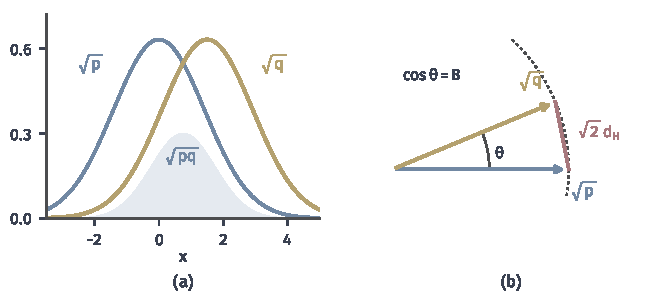
\includegraphics[width=112mm]{figures/07-probability/04-distribution-analysis/matplotlib/dcomp-hellinger-roots/figure.pdf}
 \caption{平方根密度。(a)$P=\mathcal{N}(0,1)$与$Q=\mathcal{N}(1.5,1)$的$\sqrt{p}$（蓝）与$\sqrt{q}$（黄），浅蓝区域是$\sqrt{pq}$，面积为$B\approx0.7548$。(b)例表的$\sqrt{\bm{p}}$与$\sqrt{\bm{q}}$是$\mathbb{R}^{3}$中的单位向量，画在它们张成的平面里；夹角$\theta\approx22.5^{\circ}$，$\cos\theta=B\approx0.9243$，红色弦长为$\sqrt2\,d_{\mathrm{H}}\approx0.389$。}
 \label{fig:dcomp-hellinger-roots}
\end{BookInlineFigure}

\paragraph{Bhattacharyya距离}
重叠系数的负对数
\begin{equation}
 D_{\mathrm{B}}(P,Q)=-\ln B(P,Q)
 \label{eq:dcomp-bhattacharyya-distance}
\end{equation}
称为\term{Bhattacharyya距离}（Bhattacharyya distance）。两个分布相互奇异时$B=0$，它等于$+\infty$，而$d_{\mathrm{H}}$此时只是$1$。$B$接近$1$时，$-\ln B\approx1-B=d_{\mathrm{H}}^{2}$。尽管名字里有“距离”，它不满足三角不等式。由式~\eqref{eq:dcomp-bc-gauss}，方差为$1$、均值分别为$0,1,2$的三个高斯分布两两之间的值是$\Delta^{2}/8$，于是
\[
 D_{\mathrm{B}}(\mathcal{N}(0,1),\mathcal{N}(2,1))=\frac12>\frac18+\frac18 .
\]
它随均值差平方增长，跨两步比走一步再走一步还“远”。在本章的用法里，$B$是重叠系数，$d_{\mathrm{H}}$是距离，$D_{\mathrm{B}}$只是$B$的一个单调变换。

\subsection{JS散度}
\label{sec:dcomp-js}

KL散度要求一个分布绝对连续于另一个。取$P=\operatorname{Unif}(0,1)$，$Q=\operatorname{Unif}(\tfrac12,\tfrac32)$，两个分布有一半质量重叠，可两个方向的KL散度都是$+\infty$：$P$在$(0,\tfrac12)$上有质量而$Q$没有，$Q$在$(1,\tfrac32)$上有质量而$P$没有。问题出在参考分布覆盖不到对方。一个自然的修补是换一个同时覆盖双方的参考分布，最简单的选择是两者的平均
\[
 M=\tfrac12(P+Q) .
\]
$M$的密度是$(p+q)/2$，只要$p>0$或$q>0$，它就为正。

\begin{definition}[JS散度]
\label{def:dcomp-js}
设$M=(P+Q)/2$。$P$与$Q$之间的\term{JS散度}（Jensen--Shannon divergence）是
\begin{equation}
 D_{\mathrm{JS}}(P,Q)=\frac12D_{\mathrm{KL}}(P\Vert M)+\frac12D_{\mathrm{KL}}(Q\Vert M) .
 \label{eq:dcomp-js-def}
\end{equation}
\end{definition}

用密度写出来，$\mathrm{d}P/\mathrm{d}M=2p/(p+q)$，所以
\[
 D_{\mathrm{JS}}(P,Q)=\frac12\int\Bigl(p\ln\frac{2p}{p+q}+q\ln\frac{2q}{p+q}\Bigr)\,\mathrm{d}\lambda ,
\]
其中$p=0$或$q=0$的项按$0\ln0=0$理解。

\begin{theorem}[JS散度的范围]
\label{thm:dcomp-js-range}
$D_{\mathrm{JS}}$对称，并且
\begin{equation}
 0\leq D_{\mathrm{JS}}(P,Q)\leq\ln2 .
 \label{eq:dcomp-js-range}
\end{equation}
左边等号成立当且仅当$P=Q$，右边等号成立当且仅当$P$与$Q$相互奇异。
\end{theorem}

\begin{proof}
交换$P,Q$不改变$M$，式~\eqref{eq:dcomp-js-def}的两项互换，所以对称。$P\ll M$与$Q\ll M$总成立，两项都有定义；由Gibbs不等式，两项都非负。和为零当且仅当两项都为零，即$P=M=Q$。

在$\{p>0\}$上，$2p/(p+q)\leq2$，所以
\[
 D_{\mathrm{KL}}(P\Vert M)=\int_{\{p>0\}}p\ln\frac{2p}{p+q}\,\mathrm{d}\lambda\leq\ln2,
\]
等号成立当且仅当在$\{p>0\}$上$q=0$几乎处处，即$Q(p>0)=0$。对$D_{\mathrm{KL}}(Q\Vert M)$同理，它等于$\ln2$当且仅当$P(q>0)=0$。两项都取到$\ln2$，恰好是$P$集中在$\{q=0\}$上、$Q$集中在$\{p=0\}$上，即两者相互奇异。
\end{proof}

上界$\ln2$有一个直观解释。把$P$与$Q$各以概率$\tfrac12$选出来，再按所选分布产生结果$x$，那么$x$的分布正是$M$。$D_{\mathrm{JS}}$衡量的是看到$x$后能把“选了哪一个”猜得多准；两个分布相互奇异时，看到$x$就知道答案，这一次是非题的全部不确定性$\ln2$都被消除了。这一解释将在第~\ref{chap:information-measures}章用互信息说清。

\paragraph{几个例子}
在例表上，$M=(0.45,\,0.3,\,0.25)$。两项分别是
\[
 D_{\mathrm{KL}}(P\Vert M)=0.6\ln\frac{0.6}{0.45}+0.1\ln\frac{0.1}{0.25}\approx0.0810,
\]
\[
 D_{\mathrm{KL}}(Q\Vert M)=0.3\ln\frac{0.3}{0.45}+0.4\ln\frac{0.4}{0.25}\approx0.0664 .
\]
平均得到$D_{\mathrm{JS}}(P,Q)\approx0.0737$，比上界$\ln2\approx0.6931$小得多。对开头的两个均匀分布，在重叠的$(\tfrac12,1)$上$p=q$，被积函数为零；在$(0,\tfrac12)$上只有$p=1$，被积函数是$\ln2$；在$(1,\tfrac32)$上只有$q=1$，同样是$\ln2$。于是
\[
 D_{\mathrm{JS}}(P,Q)=\frac12\Bigl(\frac12\ln2+\frac12\ln2\Bigr)=\frac12\ln2\approx0.3466 ,
\]
两个方向的KL散度都是$+\infty$，JS散度却是一个有限的数。

图~\ref{fig:dcomp-js-saturation}比较$P=\mathcal{N}(0,1)$与$Q=\mathcal{N}(\Delta,1)$。由式~\eqref{eq:dcomp-kl-gauss}，$D_{\mathrm{KL}}(P\Vert Q)=\Delta^{2}/2$，随$\Delta$无限增长；JS散度在$\Delta$较大时贴近$\ln2$，两个分布几乎不重叠以后，再拉远也几乎不再增加。JS散度有界的代价是：它分不清“已经几乎分开”与“分得非常开”。

\begin{BookInlineFigure}
 \centering
 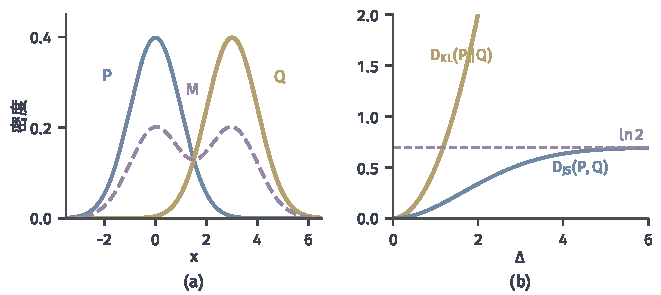
\includegraphics[width=112mm]{figures/07-probability/04-distribution-analysis/matplotlib/dcomp-js-saturation/figure.pdf}
 \caption{JS散度的饱和。(a)$P=\mathcal{N}(0,1)$（蓝）、$Q=\mathcal{N}(3,1)$（黄）与平均分布$M$（紫色虚线）。(b)$D_{\mathrm{KL}}(P\Vert Q)=\Delta^{2}/2$（黄）与$D_{\mathrm{JS}}(P,Q)$（蓝，数值积分），紫色虚线是上界$\ln2$；$\Delta=1,3,6$时JS散度依次约为$0.111$，$0.527$，$0.689$。}
 \label{fig:dcomp-js-saturation}
\end{BookInlineFigure}

\paragraph{距离性质}
JS散度对称、非负、零值只在两分布相同时取到，但它本身不满足三角不等式。在$\{0,1\}$上取$\delta_0$、$\delta_1$与均匀分布$U=(\tfrac12,\tfrac12)$。$\delta_0$与$\delta_1$相互奇异，JS散度取最大值$\ln2\approx0.6931$。$\delta_0$与$U$的平均是$(\tfrac34,\tfrac14)$，计算得
\[
 D_{\mathrm{JS}}(\delta_0,U)=\frac12\ln\frac43+\frac12\Bigl(\frac12\ln\frac23+\frac12\ln2\Bigr)=\frac34\ln\frac43\approx0.2158 .
\]
由对称性$D_{\mathrm{JS}}(U,\delta_1)$也约为$0.2158$，两者之和$0.4315$小于$0.6931$。可以证明$\sqrt{D_{\mathrm{JS}}}$满足三角不等式，因而是一个距离；证明需要把它写成某个Hilbert空间中两点的距离，篇幅较长。上例中$\sqrt{0.2158}\times2\approx0.929$，确实大于$\sqrt{0.6931}\approx0.833$。

\subsection{凸函数散度}
\label{sec:dcomp-f-divergence}

把前面几个量都写成“$Q$下对密度比的某个函数求平均”，会看到同一个形式。在$\{q>0\}$上记$t=p/q$，则
\[
 \frac12\lvert p-q\rvert=q\cdot\frac12\lvert t-1\rvert,\qquad p\ln\frac{p}{q}=q\cdot t\ln t,\qquad\frac12\bigl(\sqrt{p}-\sqrt{q}\bigr)^{2}=q\cdot\frac12\bigl(\sqrt{t}-1\bigr)^{2} .
\]
总变差、KL散度与平方Hellinger距离分别是$\int q\,f(p/q)\,\mathrm{d}\lambda$，$f$依次取$\tfrac12\lvert t-1\rvert$，$t\ln t$与$\tfrac12(\sqrt{t}-1)^{2}$。这三个函数都是凸函数，并且在$t=1$处为零，见图~\ref{fig:dcomp-f-generators}。

\begin{definition}[$f$散度]
\label{def:dcomp-f-divergence}
设$f:(0,\infty)\to\mathbb{R}$是凸函数，$f(1)=0$，并令$f(0)$为极限$\lim_{t\downarrow0}f(t)$，它可以是$+\infty$。若$P\ll Q$，定义
\begin{equation}
 D_f(P\Vert Q)=\mathbb{E}_{Q}\Bigl[f\Bigl(\frac{\mathrm{d}P}{\mathrm{d}Q}\Bigr)\Bigr]=\int_{\{q>0\}}q\,f\Bigl(\frac{p}{q}\Bigr)\,\mathrm{d}\lambda ,
 \label{eq:dcomp-f-def}
\end{equation}
称为$P$相对于$Q$的\term{$f$散度}（$f$-divergence），$f$称为它的生成函数。
\end{definition}

积分有意义：凸函数位于它的任何一条支撑线之上，存在常数$a,b$使$f(t)\geq a+bt$，所以$f(\mathrm{d}P/\mathrm{d}Q)$的负部不超过$\lvert a\rvert+\lvert b\rvert\,\mathrm{d}P/\mathrm{d}Q$，在$Q$下可积。非负性来自Jensen不等式：$\mathbb{E}_{Q}[\mathrm{d}P/\mathrm{d}Q]=1$，所以
\[
 D_f(P\Vert Q)\geq f\Bigl(\mathbb{E}_{Q}\Bigl[\frac{\mathrm{d}P}{\mathrm{d}Q}\Bigr]\Bigr)=f(1)=0 .
\]
凸性在这里起的作用，与Gibbs不等式中对数的凹性相同。

\paragraph{奇异质量}
$P$不绝对连续于$Q$时，$P$在$\{q=0\}$上有质量，那里的密度比相当于$t=+\infty$。从$\{q>0\}$一侧看，$q\,f(p/q)=p\cdot f(t)/t$，当$q\to0$而$p$固定时，它趋于$p\,f'(\infty)$，其中
\begin{equation}
 f'(\infty)=\lim_{t\to\infty}\frac{f(t)}{t}\in\mathbb{R}\cup\{+\infty\} .
 \label{eq:dcomp-f-slope-infinity}
\end{equation}
凸函数的$f(t)/t$在$t$大时单调，这个极限存在。据此把一般情形定义为
\begin{equation}
 D_f(P\Vert Q)=\int_{\{q>0\}}q\,f\Bigl(\frac{p}{q}\Bigr)\,\mathrm{d}\lambda+f'(\infty)\,P(q=0),
 \label{eq:dcomp-f-general}
\end{equation}
约定$0\cdot(+\infty)=0$。KL散度的$f'(\infty)=+\infty$，只要有奇异质量就是$+\infty$，与定义~\ref{def:dcomp-kl}一致。总变差与平方Hellinger距离的$f'(\infty)=\tfrac12$，奇异质量按一半计入：在$\{q=0\}$上$\tfrac12\lvert p-q\rvert$与$\tfrac12(\sqrt{p}-\sqrt{q})^{2}$都等于$\tfrac12p$，与直接用式~\eqref{eq:dcomp-tv-density}和式~\eqref{eq:dcomp-hellinger-def}计算的结果相同。

表~\ref{tab:dcomp-f-generators}列出常用的生成函数。JS散度也在其中：在$\{q>0\}$上把被积函数写成$q$乘以$t=p/q$的函数即得，$f'(\infty)=\tfrac12\ln2$对应于奇异部分每单位质量贡献$\tfrac12\ln2$。$\chi^{2}$散度$\int(p-q)^{2}/q\,\mathrm{d}\lambda$在例表上等于$0.09/0.3+0+0.09/0.4=0.525$。

\begin{BookInlineTable}
 \centering
 \caption{常用$f$散度的生成函数。}
 \label{tab:dcomp-f-generators}
 \begin{tabular}{lll}
  \toprule
  散度 & $f(t)$ & $f'(\infty)$\\
  \midrule
  $D_{\mathrm{KL}}(P\Vert Q)$ & $t\ln t$ & $+\infty$\\
  $D_{\mathrm{KL}}(Q\Vert P)$ & $-\ln t$ & $0$\\
  $d_{\mathrm{TV}}(P,Q)$ & $\tfrac12\lvert t-1\rvert$ & $\tfrac12$\\
  $d_{\mathrm{H}}^{2}(P,Q)$ & $\tfrac12(\sqrt{t}-1)^{2}$ & $\tfrac12$\\
  $D_{\mathrm{JS}}(P,Q)$ & $\tfrac12\bigl(t\ln\tfrac{2t}{1+t}+\ln\tfrac{2}{1+t}\bigr)$ & $\tfrac12\ln2$\\
  $\chi^{2}(P\Vert Q)$ & $(t-1)^{2}$ & $+\infty$\\
  \bottomrule
 \end{tabular}
\end{BookInlineTable}

\begin{BookInlineFigure}
 \centering
 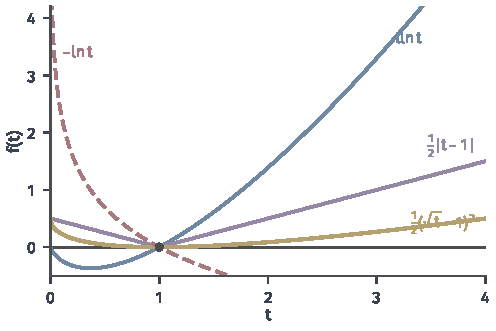
\includegraphics[width=84mm]{figures/07-probability/04-distribution-analysis/matplotlib/dcomp-f-generators/figure.pdf}
 \caption{几个生成函数在$[0,4]$上的图像：$t\ln t$（蓝，KL散度），$-\ln t$（红色虚线，反向KL散度），$\tfrac12\lvert t-1\rvert$（紫，总变差），$\tfrac12(\sqrt{t}-1)^{2}$（黄，平方Hellinger距离）。它们都是凸函数，都经过黑点$(1,0)$；右侧的斜率趋于$f'(\infty)$，决定奇异质量的计价。}
 \label{fig:dcomp-f-generators}
\end{BookInlineFigure}

表中的$-\ln t$与$t\ln t$给出两个方向的KL散度，因为在$Q$下对$-\ln(p/q)$求平均就是$D_{\mathrm{KL}}(Q\Vert P)$。一般地，$t\,f(1/t)$也是凸函数，它生成的散度是$D_f(Q\Vert P)$。生成函数也不唯一：$f(t)$与$f(t)+c(t-1)$给出同一个散度，因为附加项的贡献是$c\bigl(P(q>0)-Q(q>0)\bigr)+c\,P(q=0)=0$。

\paragraph{随机后处理}
设观测值$x$先经过一个随机处理再交给我们：给定$x$，按分布$K(x,\cdot)$产生新的结果$y$。这里$K$是第~\ref{chap:conditional-distributions}章的概率核，可以是确定的映射（$K(x,\cdot)=\delta_{T(x)}$），也可以是加噪声、四舍五入、合并类别。若原来的结果服从$P$，处理后的结果服从
\begin{equation}
 PK(B)=\int K(x,B)\,P(\mathrm{d}x),\qquad B\in\mathcal{F}_{\mathcal{Y}} .
 \label{eq:dcomp-kernel-push}
\end{equation}
直觉上，处理不会凭空增加区分$P$与$Q$的能力：任何能从$y$做出的判断，都可以先自己生成$y$再从$x$做出。下面的定理把这个直觉写成不等式。

\begin{theorem}[后处理不增加$f$散度]
\label{thm:dcomp-data-processing}
设$K$是从$\mathcal{X}$到$\mathcal{Y}$的概率核，$f$满足定义~\ref{def:dcomp-f-divergence}的条件。则
\begin{equation}
 D_f(PK\Vert QK)\leq D_f(P\Vert Q) .
 \label{eq:dcomp-data-processing}
\end{equation}
\end{theorem}

\begin{proof}
下面对$P\ll Q$的情形给出证明，这已经包含了KL散度取有限值的全部情形。若$D_f(P\Vert Q)=+\infty$，结论成立，所以设它有限。记$r=\mathrm{d}P/\mathrm{d}Q$。在一个概率空间上构造$(X,Y)$，使$X\sim Q$，给定$X=x$时$Y$的条件分布是$K(x,\cdot)$，于是$Y\sim QK$。

先找出$PK$相对于$QK$的密度。对$B\in\mathcal{F}_{\mathcal{Y}}$，由式~\eqref{eq:dcomp-kernel-push}与$r$的定义，再对$X$取条件，
\[
 PK(B)=\mathbb{E}\bigl[r(X)K(X,B)\bigr]=\mathbb{E}\bigl[r(X)\mathbf{1}_{\{Y\in B\}}\bigr]=\mathbb{E}\bigl[s(Y)\mathbf{1}_{\{Y\in B\}}\bigr],
\]
其中$s(Y)=\mathbb{E}[r(X)\mid Y]$，最后一步是条件期望的定义；$s$是可测函数，由第~\ref{chap:conditional-expectation}章，条件期望可以写成$Y$的函数。上式说明$PK\ll QK$，并且$s$就是$\mathrm{d}(PK)/\mathrm{d}(QK)$。

于是左边的散度是$\mathbb{E}[f(s(Y))]$。对凸函数$f$用条件Jensen不等式，再用全期望公式，
\[
 \mathbb{E}\bigl[f(\mathbb{E}[r(X)\mid Y])\bigr]\leq\mathbb{E}\bigl[\mathbb{E}[f(r(X))\mid Y]\bigr]=\mathbb{E}\bigl[f(r(X))\bigr]=D_f(P\Vert Q) .
\]
第~\ref{chap:conditional-expectation}章的条件Jensen不等式对定义在$\mathbb{R}$上的凸函数陈述；$f$定义在$[0,\infty)$上，$r\geq0$，证明只用到可数条支撑线，对这里的$f$同样成立。$f(r(X))$可积，因为$D_f(P\Vert Q)$有限且负部可积。
\end{proof}

$P$不绝对连续于$Q$的情形可以用同样的思路证明：取$\lambda=(P+Q)/2$，把两个密度$(\mathrm{d}P/\mathrm{d}\lambda,\mathrm{d}Q/\mathrm{d}\lambda)$一起作为二维随机向量，对二元凸函数$(a,b)\mapsto b\,f(a/b)$使用条件Jensen不等式。步骤与上面相同，只是要另外讨论$b=0$的边界。

证明的核心是一句话：处理后的密度比是处理前密度比的条件平均，而对凸函数先平均再作用，结果不超过先作用再平均。条件平均把不同$x$上的密度比混在一起，比值的起伏被抹平，凸函数度量的“偏离$1$的程度”只能变小。

\paragraph{合并类别}
在例表上做确定的合并。把$1$与$2$合并成一类，两份表变成$(0.6,0.4)$与$(0.3,0.7)$，KL散度从$0.2773$降到
\[
 0.6\ln\frac{0.6}{0.3}+0.4\ln\frac{0.4}{0.7}\approx0.1920 ,
\]
总变差仍是$0.3$。总变差不变，是因为合并后仍能区分最坏事件$A^{*}=\{0\}$。若改把$0$与$2$合并，两份表都变成$(0.7,0.3)$，所有散度都变成零：点$0$处$P$多出的$0.3$与点$2$处$Q$多出的$0.3$被并到同一类里，正好抵消，区分两个分布的信息全部丢失。图~\ref{fig:dcomp-merging}画出这三种情况。

\begin{BookInlineFigure}
 \centering
 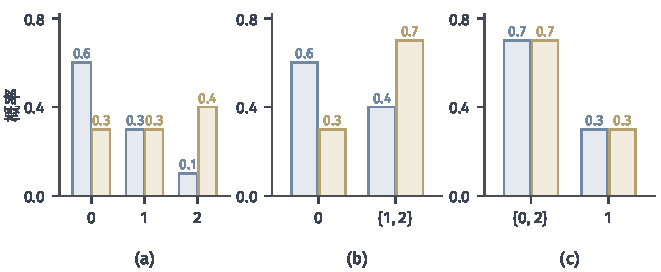
\includegraphics[width=112mm]{figures/07-probability/04-distribution-analysis/matplotlib/dcomp-merging/figure.pdf}
 \caption{确定性后处理对例表的影响，蓝色为$P$，黄色为$Q$。(a)原表：$d_{\mathrm{TV}}=0.3$，$D_{\mathrm{KL}}(P\Vert Q)\approx0.2773$。(b)合并$1$与$2$：$d_{\mathrm{TV}}=0.3$，$D_{\mathrm{KL}}\approx0.1920$。(c)合并$0$与$2$：两表相同，所有散度为零。}
 \label{fig:dcomp-merging}
\end{BookInlineFigure}

若$T$是可测的一一映射且逆映射也可测，对$T$与$T^{-1}$各用一次式~\eqref{eq:dcomp-data-processing}，得到$D_f$在$T$下不变。重新标号、单位换算这类可逆变换不改变任何$f$散度。

\subsection{Rényi散度}
\label{sec:dcomp-renyi}

KL散度按$P$的权重平均对数比。另一种做法是对密度比取幂：在$\{q>0\}$上，
\[
 \int p^{\alpha}q^{1-\alpha}\,\mathrm{d}\lambda=\mathbb{E}_{Q}\Bigl[\Bigl(\frac{p}{q}\Bigr)^{\alpha}\Bigr] .
\]
阶数$\alpha>1$时，幂函数放大大的比值，散度主要由“$P$比$Q$多出很多”的位置决定；$\alpha<1$时放大作用变弱。取对数并归一化，就得到一族以$\alpha$为参数的比较量。

\begin{definition}[Rényi散度]
\label{def:dcomp-renyi}
设$\alpha\in(0,1)\cup(1,\infty)$，$p,q$是相对于共同支配测度$\lambda$的密度。$P$相对于$Q$的$\alpha$阶\term{Rényi散度}（Rényi divergence）是
\begin{equation}
 D_{\alpha}(P\Vert Q)=\frac{1}{\alpha-1}\ln\int p^{\alpha}q^{1-\alpha}\,\mathrm{d}\lambda ,
 \label{eq:dcomp-renyi-def}
\end{equation}
其中被积函数在$p=0$处取$0$；$\alpha>1$时，在$q=0<p$处取$+\infty$。
\end{definition}

零密度的约定决定了无穷值何时出现。$\alpha>1$时，$q^{1-\alpha}$在$q\to0$时趋于无穷，只要$P(q=0)>0$，积分就是$+\infty$，散度为$+\infty$，这与KL散度要求$P\ll Q$一致。$\alpha<1$时，$q^{1-\alpha}\to0$，奇异质量对积分没有贡献；积分为$0$当且仅当$pq=0$几乎处处，即两个分布相互奇异，此时$\ln0=-\infty$除以负数$\alpha-1$，散度同样为$+\infty$。与Hellinger距离一样，被积函数关于密度一次齐次，结果与$\lambda$的选取无关。

两个特殊阶数与前面的量直接对应。$\alpha=\tfrac12$时积分是Bhattacharyya系数，$\alpha=2$时积分是$\int p^{2}/q\,\mathrm{d}\lambda$，它等于$1+\chi^{2}(P\Vert Q)$，所以
\begin{equation}
 D_{1/2}(P\Vert Q)=-2\ln B(P,Q),\qquad D_{2}(P\Vert Q)=\ln\bigl(1+\chi^{2}(P\Vert Q)\bigr) .
 \label{eq:dcomp-renyi-special}
\end{equation}
在例表上，由$B\approx0.9243$与$\chi^{2}=0.525$，
\[
 D_{1/2}\approx0.1575,\qquad D_{\mathrm{KL}}\approx0.2773,\qquad D_{2}=\ln1.525\approx0.4220 .
\]
KL散度恰好夹在中间。图~\ref{fig:dcomp-renyi-order}画出$D_{\alpha}$随$\alpha$的变化，它是一条单调上升的曲线，在$\alpha=1$处连续地经过KL散度。

\begin{BookInlineFigure}
 \centering
 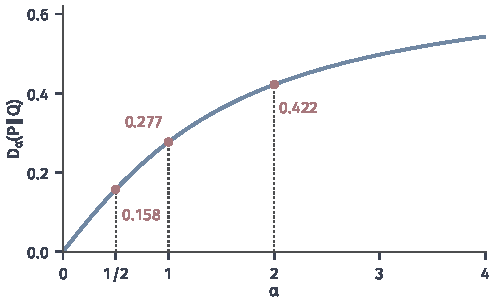
\includegraphics[width=84mm]{figures/07-probability/04-distribution-analysis/matplotlib/dcomp-renyi-order/figure.pdf}
 \caption{例表的Rényi散度$D_{\alpha}(P\Vert Q)$随阶数$\alpha$的变化（蓝）。红点依次是$\alpha=\tfrac12$处的$-2\ln B\approx0.158$，$\alpha=1$处的KL散度$0.4\ln2\approx0.277$，$\alpha=2$处的$\ln(1+\chi^{2})\approx0.422$。}
 \label{fig:dcomp-renyi-order}
\end{BookInlineFigure}

\begin{theorem}[阶数的单调性与KL极限]
\label{thm:dcomp-renyi-order}
对$0<\alpha<1<\beta$，
\begin{equation}
 D_{\alpha}(P\Vert Q)\leq D_{\mathrm{KL}}(P\Vert Q)\leq D_{\beta}(P\Vert Q),
 \label{eq:dcomp-renyi-sandwich}
\end{equation}
并且$\alpha\mapsto D_{\alpha}(P\Vert Q)$在$(0,1)$与$(1,\infty)$上都单调不减，$\alpha\uparrow1$时$D_{\alpha}(P\Vert Q)\to D_{\mathrm{KL}}(P\Vert Q)$。
\end{theorem}

\begin{proof}
若$P$不绝对连续于$Q$，则$D_{\mathrm{KL}}$与所有$\beta>1$的$D_{\beta}$都是$+\infty$，不等式与右侧的单调性成立；左侧的论证不用绝对连续，放在下面一并处理。先设$P\ll Q$。

\emph{改写成幂平均。}在$\{p>0\}$上令$R=q/p$，它在$P$下几乎处处取正的有限值。被积函数在$p=0$处为零，所以
\[
 \int p^{\alpha}q^{1-\alpha}\,\mathrm{d}\lambda=\int_{\{p>0\}}p\,R^{1-\alpha}\,\mathrm{d}\lambda=\mathbb{E}_{P}\bigl[R^{s}\bigr],\qquad s=1-\alpha .
\]
对$s\neq0$记$M_s=(\mathbb{E}_{P}[R^{s}])^{1/s}$，称为$R$的$s$次幂平均，再记$M_0=\exp(\mathbb{E}_{P}[\ln R])$。由式~\eqref{eq:dcomp-renyi-def}与式~\eqref{eq:dcomp-kl-def}，
\[
 D_{\alpha}(P\Vert Q)=-\ln M_{1-\alpha},\qquad D_{\mathrm{KL}}(P\Vert Q)=-\mathbb{E}_{P}[\ln R]=-\ln M_0 .
\]
$\alpha$增大时$s$减小，所以只需证明$M_s$关于$s$单调不减。

\emph{幂平均的单调性。}对$0<s<t$，函数$u\mapsto u^{t/s}$在$[0,\infty)$上凸，由Jensen不等式，
\[
 \bigl(\mathbb{E}_{P}[R^{s}]\bigr)^{t/s}\leq\mathbb{E}_{P}[R^{t}],
\]
开$t$次方得$M_s\leq M_t$。对$s<t<0$，把同一结论用于$1/R$与指数$-t<-s$，取倒数即得。对$s<0<t$，由对数的凹性，
\[
 t\,\mathbb{E}_{P}[\ln R]\leq\ln\mathbb{E}_{P}[R^{t}],\qquad s\,\mathbb{E}_{P}[\ln R]\leq\ln\mathbb{E}_{P}[R^{s}] .
\]
第一式除以$t>0$得$\ln M_0\leq\ln M_t$；第二式除以$s<0$，不等号反向，得$\ln M_0\geq\ln M_s$。于是$M_s\leq M_0\leq M_t$，这就是式~\eqref{eq:dcomp-renyi-sandwich}与两段上的单调性。$\mathbb{E}_{P}[R^{s}]=+\infty$（$s<0$时可能发生）时$M_s=0$，对应的散度为$+\infty$，不等式仍成立。

\emph{左侧的极限。}令$\alpha\uparrow1$，即$s\downarrow0$。对固定的$R>0$，$s\mapsto R^{s}$是凸函数，差商$(R^{s}-1)/s$随$s$减小而单调下降，极限是$\ln R$；$s=1$时差商为$R-1$，在$P$下可积。由单调收敛定理（单调下降、首项可积），
\[
 a_s=\mathbb{E}_{P}\Bigl[\frac{R^{s}-1}{s}\Bigr]\downarrow\mathbb{E}_{P}[\ln R]=-D_{\mathrm{KL}}(P\Vert Q) .
\]
而$\mathbb{E}_{P}[R^{s}]=1+s\,a_s$，所以
\[
 -D_{\alpha}(P\Vert Q)=\frac{1}{s}\ln\mathbb{E}_{P}[R^{s}]=\frac{\ln(1+s\,a_s)}{s} .
\]
若$D_{\mathrm{KL}}$有限，$s\,a_s\to0$，$\ln(1+u)/u\to1$，所以$-D_{\alpha}\to-D_{\mathrm{KL}}$。若$D_{\mathrm{KL}}=+\infty$，由$\ln(1+u)\leq u$得$-D_{\alpha}\leq a_s\to-\infty$。两种情形都有$D_{\alpha}\to D_{\mathrm{KL}}$。

最后，$P$不绝对连续于$Q$时，把$R$在$\{q=0<p\}$上定义为$0$，上面关于$s\in(0,1)$的改写和左侧的极限论证照样成立，结论是$D_{\alpha}\to+\infty=D_{\mathrm{KL}}$。
\end{proof}

\paragraph{另一侧的极限需要条件}
$\alpha\downarrow1$时，$D_{\beta}$未必趋于KL散度。在正整数上取
\[
 p_k=c\,k^{-3},\qquad q_k=(\mathrm{e}-1)\,\mathrm{e}^{-k},\qquad k=1,2,\dots,
\]
其中$c=1/\sum_kk^{-3}\approx0.8319$。对数比$\ln(p_k/q_k)$约按$k$线性增长，而$p_k$按$k^{-3}$衰减，所以$D_{\mathrm{KL}}(P\Vert Q)=\sum_kp_k\ln(p_k/q_k)$收敛，数值约为$0.1446$。但对任何$\beta>1$，
\[
 p_k^{\beta}q_k^{1-\beta}=c^{\beta}(\mathrm{e}-1)^{1-\beta}\,k^{-3\beta}\,\mathrm{e}^{(\beta-1)k}\to+\infty,
\]
级数发散，$D_{\beta}(P\Vert Q)=+\infty$。比值$p_k/q_k$的增长是指数型的，任何正次幂都会让它压过$p_k$的多项式衰减，而对数只把它变成线性增长。若存在某个$\beta>1$使$D_{\beta}$有限，那么$\alpha\downarrow1$时$D_{\alpha}\to D_{\mathrm{KL}}$，证明与上面类似，用支配收敛定理代替单调收敛定理。

\paragraph{与$f$散度的关系}
令$f_{\alpha}(t)=(t^{\alpha}-1)/(\alpha-1)$。$\alpha>1$时$t^{\alpha}$凸，除以正数；$\alpha<1$时$t^{\alpha}$凹，除以负数，所以$f_{\alpha}$总是凸函数，并且$f_{\alpha}(1)=0$。它生成的$f$散度记作$H_{\alpha}$，对比式~\eqref{eq:dcomp-renyi-def}，
\[
 D_{\alpha}(P\Vert Q)=\frac{1}{\alpha-1}\ln\bigl(1+(\alpha-1)H_{\alpha}(P\Vert Q)\bigr) .
\]
右边是$H_{\alpha}$的单调增函数，所以定理~\ref{thm:dcomp-data-processing}立即给出：后处理也不增加Rényi散度。

单调变换保住了大小顺序，却改变了结构，$D_{\alpha}$本身一般不是$f$散度。任何$f$散度在不交区域上按权相加：若$P=\tfrac12P_1+\tfrac12P_2$，$Q=\tfrac12Q_1+\tfrac12Q_2$，并且$P_1,Q_1$集中在$A$上，$P_2,Q_2$集中在$A^{\mathrm{c}}$上，把式~\eqref{eq:dcomp-f-general}的积分拆到$A$与$A^{\mathrm{c}}$上就得到
\[
 D_f(P\Vert Q)=\tfrac12D_f(P_1\Vert Q_1)+\tfrac12D_f(P_2\Vert Q_2) .
\]
在$\{0,1,2\}$上取$A=\{0,1\}$与
\[
 P=(\tfrac12,\ 0,\ \tfrac12),\qquad Q=(\tfrac14,\ \tfrac14,\ \tfrac12) .
\]
按上面的分解，$P_1=(1,0)$与$Q_1=(\tfrac12,\tfrac12)$在$A$上，$P_2,Q_2$都是$\delta_2$。直接计算，
\[
 D_2(P\Vert Q)=\ln\Bigl(\frac{1/4}{1/4}+\frac{1/4}{1/2}\Bigr)=\ln1.5\approx0.4055,
\]
而按块加权的结果是
\[
 \tfrac12D_2(P_1\Vert Q_1)+\tfrac12D_2(P_2\Vert Q_2)=\tfrac12\ln2+0\approx0.3466 .
\]
两者不等，所以不存在$f$使$D_2=D_f$对所有分布对成立。作为对照，KL散度满足这个可加性：$D_{\mathrm{KL}}(P\Vert Q)$与$\tfrac12D_{\mathrm{KL}}(P_1\Vert Q_1)$都等于$\tfrac12\ln2$。

\section{基于测试函数的比较}
\label{sec:dcomp-ipm}

密度比较要求两个分布写在同一个支配测度下，并且只看同一位置上的取值。另一种做法不碰密度，只看两个分布对一些函数给出的平均。选定一个函数$g$，读出$\mathbb{E}_{P}[g]$与$\mathbb{E}_{Q}[g]$，两者的差就是用$g$这把“尺子”量到的差异。用一族尺子同时去量，取最大的读数差，就得到一个比较量。式~\eqref{eq:dcomp-tv-dual}已经是这种形式：总变差是有界函数单位球上的最大期望差。这里要回答的是：换成别的函数类会得到什么，函数类要多丰富才能分辨所有不同的分布，以及怎样实际算出上确界。

\subsection{函数类与可辨别差异}
\label{sec:dcomp-ipm-classes}

\begin{definition}[积分概率度量]
\label{def:dcomp-ipm}
设$\mathcal{G}$是一族$\mathcal{X}$上的实值可测函数，其中每个$g$在$P$与$Q$下都可积。称
\begin{equation}
 d_{\mathcal{G}}(P,Q)=\sup_{g\in\mathcal{G}}\bigl\lvert\mathbb{E}_{P}[g]-\mathbb{E}_{Q}[g]\bigr\rvert
 \label{eq:dcomp-ipm-def}
\end{equation}
为由$\mathcal{G}$生成的\term{积分概率度量}（integral probability metric）。
\end{definition}

这个量对称，并且满足三角不等式：对第三个分布$R$与每个$g$，
\[
 \lvert\mathbb{E}_{P}g-\mathbb{E}_{R}g\rvert\leq\lvert\mathbb{E}_{P}g-\mathbb{E}_{Q}g\rvert+\lvert\mathbb{E}_{Q}g-\mathbb{E}_{R}g\rvert ,
\]
再对$g$取上确界。定义要检查两件事。

第一，上确界是否有限。若$\mathcal{G}$对数乘封闭，例如取全体有界可测函数而不限制大小，只要某个$g$的读数差不为零，把$g$放大$c$倍读数差就放大$c$倍，上确界是$+\infty$。所以函数类通常要带一个范数约束，如$\lVert g\rVert_{\infty}\leq1$。

第二，零值能否辨别分布。比较量为零只说明$P$与$Q$在$\mathcal{G}$中每个函数上的平均相同。若$\mathcal{G}$太小，不同的分布也可能得到零。取$\mathcal{G}$只含$x$与$x^{2}$两个函数，它只比较均值与二阶矩。标准高斯分布$P$与区间$(-\sqrt3,\sqrt3)$上的均匀分布$Q$的均值都是$0$，二阶矩都是$1$，所以这个函数类给出的比较量为零，两个分布却明显不同，见图~\ref{fig:dcomp-moment-matching}。一旦加入$\cos x$或$\mathbf{1}_{\{\lvert x\rvert\leq1\}}$这样的函数，差异立即显现：
\[
 \mathbb{E}_{P}[\cos X]-\mathbb{E}_{Q}[\cos X]=\mathrm{e}^{-1/2}-\frac{\sin\sqrt3}{\sqrt3}\approx0.0367,
\]
\[
 P(\lvert X\rvert\leq1)-Q(\lvert X\rvert\leq1)=\bigl(2\Phi(1)-1\bigr)-\frac{1}{\sqrt3}\approx0.1053 .
\]

\begin{BookInlineFigure}
 \centering
 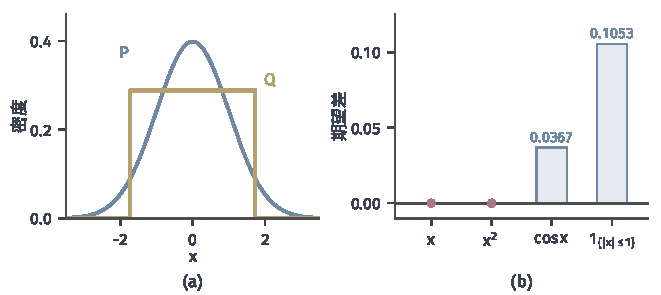
\includegraphics[width=112mm]{figures/07-probability/04-distribution-analysis/matplotlib/dcomp-moment-matching/figure.pdf}
 \caption{函数类决定能看到的差异。(a)$P=\mathcal{N}(0,1)$（蓝）与$Q=\operatorname{Unif}(-\sqrt3,\sqrt3)$（黄），均值都是$0$，方差都是$1$。(b)四个测试函数上的期望差$\mathbb{E}_{P}[g]-\mathbb{E}_{Q}[g]$：$x$与$x^{2}$为零（红点），$\cos x$与$\mathbf{1}_{\{\lvert x\rvert\leq1\}}$不为零。}
 \label{fig:dcomp-moment-matching}
\end{BookInlineFigure}

几种常见的函数类各有含义。有界函数单位球给出$2d_{\mathrm{TV}}$，能辨别任何两个不同的分布，但对位置的微小移动同样“看得见”，见第~\ref{sec:dcomp-tv-definition}节末尾。$\mathbb{R}$上半直线的示性函数$\mathbf{1}_{(-\infty,t]}$给出$\sup_t\lvert F_P(t)-F_Q(t)\rvert$，称为\term{Kolmogorov距离}（Kolmogorov distance）；分布函数决定分布，所以它也能辨别分布。$\mathbb{R}^{d}$上的全体有界连续函数也能辨别分布，这是第~\ref{chap:weak-convergence-of-distributions}章中弱收敛极限唯一的依据。1-Lipschitz函数类给出第~\ref{sec:dcomp-wasserstein}节的一阶Wasserstein距离。

函数类越大，比较越严格，但上确界也越难计算：对一般的函数类，要在无穷维集合上求最大值。下面构造一类函数，使上确界有闭式解。

\subsection{核均值}
\label{sec:dcomp-kernel-mean}

取再生核Hilbert空间（RKHS）的单位球作为函数类。设$k$是$\mathcal{X}$上的正定核，$\mathcal{H}$是它的RKHS，内积记作$\langle\cdot,\cdot\rangle_{\mathcal{H}}$。卷四给出了它的基本性质：每个$x$对应一个函数$k(x,\cdot)\in\mathcal{H}$，并且对一切$g\in\mathcal{H}$，
\begin{equation}
 g(x)=\bigl\langle g,\,k(x,\cdot)\bigr\rangle_{\mathcal{H}},\qquad\bigl\lVert k(x,\cdot)\bigr\rVert_{\mathcal{H}}=\sqrt{k(x,x)},
 \label{eq:dcomp-reproducing}
\end{equation}
可参考\BookChapterRef{chap:rkhs}{卷四第23章“再生核Hilbert空间”}。映射$x\mapsto k(x,\cdot)$是特征映射，它把$\mathcal{X}$中的点放进Hilbert空间。为避免与概率核混淆，本节的核用小写$k$。

再生性质~\eqref{eq:dcomp-reproducing}把求值变成内积。若在两边对$X\sim P$取期望，并把期望移进内积里，就得到
\[
 \mathbb{E}_{P}[g(X)]=\bigl\langle g,\ \mathbb{E}_{P}[k(X,\cdot)]\bigr\rangle_{\mathcal{H}} .
\]
右边的$\mathbb{E}_{P}[k(X,\cdot)]$是特征点的平均位置，也就是把单位质量按$P$放到这些特征点上之后的重心。下面的定理说明这个重心在什么条件下存在，并绕开“向量值期望”的定义，直接用内积刻画它。

\begin{theorem}[核均值]
\label{thm:dcomp-kernel-mean}
设$\mathcal{H}$可分，特征映射$x\mapsto k(x,\cdot)$可测，并且
\begin{equation}
 \mathbb{E}_{P}\Bigl[\sqrt{k(X,X)}\Bigr]<\infty .
 \label{eq:dcomp-kernel-moment}
\end{equation}
则每个$g\in\mathcal{H}$在$P$下可积，并且存在唯一的$m_P\in\mathcal{H}$，使
\begin{equation}
 \mathbb{E}_{P}[g(X)]=\langle g,m_P\rangle_{\mathcal{H}},\qquad g\in\mathcal{H} .
 \label{eq:dcomp-kernel-mean}
\end{equation}
它的取值是$m_P(y)=\mathbb{E}_{P}[k(X,y)]$。
\end{theorem}

\begin{proof}
对$g\in\mathcal{H}$，$g(x)=\langle g,k(x,\cdot)\rangle_{\mathcal{H}}$是连续线性泛函与可测映射的复合，所以$g$可测。由Cauchy--Schwarz不等式与式~\eqref{eq:dcomp-reproducing}，
\[
 \lvert g(x)\rvert\leq\lVert g\rVert_{\mathcal{H}}\sqrt{k(x,x)} .
\]
由条件~\eqref{eq:dcomp-kernel-moment}，$g$在$P$下可积，并且线性泛函$L(g)=\mathbb{E}_{P}[g(X)]$满足
\[
 \lvert L(g)\rvert\leq\mathbb{E}_{P}\Bigl[\sqrt{k(X,X)}\Bigr]\,\lVert g\rVert_{\mathcal{H}},
\]
是有界线性泛函。由Riesz表示定理，存在唯一的$m_P\in\mathcal{H}$使$L(g)=\langle g,m_P\rangle_{\mathcal{H}}$，可参考\BookChapterRef{chap:function-inner-product-spaces}{卷四第12章“内积空间”}。取$g=k(y,\cdot)$，由式~\eqref{eq:dcomp-reproducing}，左边是$\mathbb{E}_{P}[k(X,y)]$，右边是$m_P(y)$。
\end{proof}

$m_P$称为$P$的\term{核均值}（kernel mean embedding），映射$P\mapsto m_P$把概率分布表示为$\mathcal{H}$中的元素。可分性在这里的作用是保证可测性在两种意义下一致：可分Hilbert空间中，“每个$g(x)=\langle g,k(x,\cdot)\rangle$都可测”与“特征映射作为Hilbert空间值映射可测”是等价的，所以定理的条件可以按任一种理解检查。条件~\eqref{eq:dcomp-kernel-moment}是特征点到原点距离的一阶矩，有界核（如高斯核，$k(x,x)=1$）对任何分布都满足它。这一节新增的只是“分布的表示”，RKHS本身仍是卷四的对象。

\paragraph{例表上的核均值}
在例表上取$\sigma=1$的高斯核$k(x,y)=\exp(-(x-y)^{2}/2)$。分布有限时期望就是加权和，
\[
 m_P=\sum_{i}p_i\,k(x_i,\cdot)=0.6\,k(0,\cdot)+0.3\,k(1,\cdot)+0.1\,k(2,\cdot) .
\]
它是三个以$0,1,2$为中心的高斯隆起按概率加权之和，见图~\ref{fig:dcomp-kernel-mean}(a)中的点线。在三个支撑点上，
\[
 m_P(0)\approx0.7955,\qquad m_P(1)\approx0.7246,\qquad m_P(2)\approx0.3632,
\]
\[
 m_Q(0)\approx0.5361,\qquad m_Q(1)\approx0.7246,\qquad m_Q(2)\approx0.6226 .
\]
核均值是概率质量用核“抹开”后的形状。$P$的质量偏左，$m_P$的峰也偏左。

\subsection{MMD}
\label{sec:dcomp-mmd}

有了核均值，RKHS单位球上的最大期望差就是一个Hilbert空间中的最大内积问题，答案由Cauchy--Schwarz不等式直接给出。

\begin{theorem}[MMD的表示]
\label{thm:dcomp-mmd}
设$P,Q$都满足条件~\eqref{eq:dcomp-kernel-moment}。则
\begin{equation}
 \operatorname{MMD}_k(P,Q)=\sup_{\lVert g\rVert_{\mathcal{H}}\leq1}\bigl\lvert\mathbb{E}_{P}[g]-\mathbb{E}_{Q}[g]\bigr\rvert=\lVert m_P-m_Q\rVert_{\mathcal{H}} .
 \label{eq:dcomp-mmd-def}
\end{equation}
设$X,X'\sim P$，$Y,Y'\sim Q$，四者相互独立，则
\begin{equation}
 \operatorname{MMD}_k^{2}(P,Q)=\mathbb{E}\bigl[k(X,X')\bigr]-2\,\mathbb{E}\bigl[k(X,Y)\bigr]+\mathbb{E}\bigl[k(Y,Y')\bigr] .
 \label{eq:dcomp-mmd-kernel}
\end{equation}
\end{theorem}

\begin{proof}
由式~\eqref{eq:dcomp-kernel-mean}，
\[
 \mathbb{E}_{P}[g]-\mathbb{E}_{Q}[g]=\langle g,m_P-m_Q\rangle_{\mathcal{H}} .
\]
由Cauchy--Schwarz不等式，单位球上它的绝对值不超过$\lVert m_P-m_Q\rVert_{\mathcal{H}}$；若$m_P\neq m_Q$，取$m_P-m_Q$方向上的单位向量$g^{*}$即可达到，若相等则两边都是零。这证明了式~\eqref{eq:dcomp-mmd-def}。

展开平方范数，
\[
 \lVert m_P-m_Q\rVert_{\mathcal{H}}^{2}=\langle m_P,m_P\rangle_{\mathcal{H}}-2\langle m_P,m_Q\rangle_{\mathcal{H}}+\langle m_Q,m_Q\rangle_{\mathcal{H}} .
\]
对中间一项，把式~\eqref{eq:dcomp-kernel-mean}用于$g=m_P$与分布$Q$，再用$m_P(y)=\mathbb{E}_{P}[k(X,y)]$，
\[
 \langle m_P,m_Q\rangle_{\mathcal{H}}=\mathbb{E}_{Q}\bigl[m_P(Y)\bigr]=\mathbb{E}\bigl[k(X,Y)\bigr] .
\]
最后一步是对独立的$(X,Y)$用Fubini定理，所需的可积性来自$\lvert k(x,y)\rvert\leq\sqrt{k(x,x)k(y,y)}$与条件~\eqref{eq:dcomp-kernel-moment}。另两项同理。
\end{proof}

\term{最大均值差异}（maximum mean discrepancy）这个名字来自式~\eqref{eq:dcomp-mmd-def}的左端，简称MMD。达到上确界的$g^{*}$称为\term{见证函数}（witness function），它在$P$质量多于$Q$的地方取正值，在少于$Q$的地方取负值，是RKHS单位球中最能“看出”两者差别的那把尺子。式~\eqref{eq:dcomp-mmd-kernel}把无穷维的上确界化成了三个核期望：同一分布内两点的平均相似度，减去跨分布两点的平均相似度的两倍。

\paragraph{例表上的计算}
继续用$\sigma=1$的高斯核。记$\bm{K}$为$3\times3$矩阵，$\bm{K}_{i,j}=k(i-1,j-1)$，即$\exp(-(i-j)^{2}/2)$。三个核期望是二次型，
\[
 \bm{p}^{\top}\bm{K}\bm{p}\approx0.7310,\qquad\bm{p}^{\top}\bm{K}\bm{q}\approx0.6013,\qquad\bm{q}^{\top}\bm{K}\bm{q}\approx0.6272 .
\]
由式~\eqref{eq:dcomp-mmd-kernel}，
\[
 \operatorname{MMD}_k^{2}(P,Q)\approx0.7310-2\times0.6013+0.6272=0.1556 .
\]
也可以直接用$\bm{p}-\bm{q}=(0.3,0,-0.3)^{\top}$计算二次型：
\[
 (\bm{p}-\bm{q})^{\top}\bm{K}(\bm{p}-\bm{q})=0.09\,(1+1-2\mathrm{e}^{-2})=0.18(1-\mathrm{e}^{-2})\approx0.1556 .
\]
开方得$\operatorname{MMD}_k(P,Q)\approx0.3945$。见证函数在三个支撑点上的值是$0.6575$，$0$，$-0.6575$，代入
\[
 \begin{aligned}
 \mathbb{E}_{P}[g^{*}]-\mathbb{E}_{Q}[g^{*}]&=\sum_i(p_i-q_i)\,g^{*}(x_i)\\
 &=0.3\times0.6575+(-0.3)\times(-0.6575)\approx0.3945 ,
 \end{aligned}
\]
与MMD相等，见图~\ref{fig:dcomp-kernel-mean}(b)。

\begin{BookInlineFigure}
 \centering
 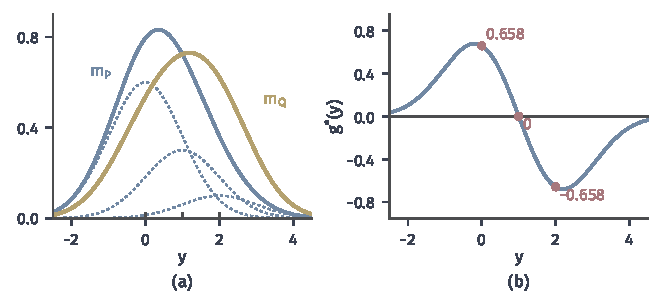
\includegraphics[width=112mm]{figures/07-probability/04-distribution-analysis/matplotlib/dcomp-kernel-mean/figure.pdf}
 \caption{例表的核均值，高斯核$\sigma=1$。(a)$m_P$（蓝）与$m_Q$（黄）；蓝色点线是三个加权核截面$p_i\,k(x_i,\cdot)$，深灰短线标出支撑点$0,1,2$。(b)见证函数$g^{*}=(m_P-m_Q)/\operatorname{MMD}_k$，红点是它在支撑点上的值。}
 \label{fig:dcomp-kernel-mean}
\end{BookInlineFigure}

式~\eqref{eq:dcomp-mmd-kernel}是两个总体分布之间的量。实际中常常只有两组样本，把期望换成样本平均就得到估计值；估计的偏差、方差与检验属于卷八的内容，这里只讨论总体量本身。

\subsection{核的辨别能力}
\label{sec:dcomp-characteristic}

MMD为零意味着$m_P=m_Q$。核均值是否把不同的分布映到不同的元素，取决于核。

\begin{definition}[特征核]
\label{def:dcomp-characteristic}
设$\mathcal{P}_k$是满足条件~\eqref{eq:dcomp-kernel-moment}的全体概率分布。若映射$P\mapsto m_P$在$\mathcal{P}_k$上是单射，则称$k$为\term{特征核}（characteristic kernel）。
\end{definition}

由式~\eqref{eq:dcomp-mmd-def}，$k$是特征核当且仅当对$\mathcal{P}_k$中的分布，$\operatorname{MMD}_k(P,Q)=0$等价于$P=Q$。不是特征核的例子很容易造。线性核$k(x,y)=xy$的RKHS只含线性函数，$m_P(y)=y\,\mathbb{E}_{P}[X]$，MMD只比较均值。二次核$k(x,y)=(1+xy)^{2}$的核均值是
\[
 m_P(y)=\mathbb{E}_{P}\bigl[(1+Xy)^{2}\bigr]=1+2y\,\mathbb{E}_{P}[X]+y^{2}\,\mathbb{E}_{P}[X^{2}],
\]
它只记录前两阶矩。图~\ref{fig:dcomp-moment-matching}中的两个分布在这个核下MMD为零。高斯核则不同。

在$\mathbb{R}^{d}$上取带宽$\sigma>0$的高斯核
\begin{equation}
 k_\sigma(\bm{x},\bm{y})=\exp\Bigl(-\frac{\lVert\bm{x}-\bm{y}\rVert_2^{2}}{2\sigma^{2}}\Bigr) .
 \label{eq:dcomp-gauss-kernel}
\end{equation}
它的谱表示把MMD与特征函数联系起来。

\begin{theorem}[高斯核的谱表示]
\label{thm:dcomp-gauss-characteristic}
设$k_\sigma$如式~\eqref{eq:dcomp-gauss-kernel}，$\Lambda_\sigma$是协方差矩阵为$\sigma^{-2}\bm{I}$的中心高斯分布。对$\mathbb{R}^{d}$上任意概率分布$P,Q$，
\begin{equation}
 \operatorname{MMD}_{k_\sigma}^{2}(P,Q)=\int_{\mathbb{R}^{d}}\bigl\lvert\phi_P(\bm{\omega})-\phi_Q(\bm{\omega})\bigr\rvert^{2}\,\Lambda_\sigma(\mathrm{d}\bm{\omega}),
 \label{eq:dcomp-mmd-spectral}
\end{equation}
其中$\phi_P,\phi_Q$是两个分布的特征函数。因此$k_\sigma$是特征核。
\end{theorem}

\begin{proof}
设$\bm{W}\sim\Lambda_\sigma$。高斯分布的特征函数给出，对任意$\bm{u}\in\mathbb{R}^{d}$，
\[
 \mathbb{E}\bigl[\mathrm{e}^{\mathrm{i}\langle\bm{W},\bm{u}\rangle}\bigr]=\exp\Bigl(-\frac{\lVert\bm{u}\rVert_2^{2}}{2\sigma^{2}}\Bigr)=k_\sigma(\bm{x},\bm{y}),\qquad\bm{u}=\bm{x}-\bm{y} .
\]
取$\bm{X}\sim P$，$\bm{Y}\sim Q$与$\bm{W}$相互独立。被积函数的模为$1$，由Fubini定理可以先对$\bm{X},\bm{Y}$积分：
\[
 \mathbb{E}\bigl[k_\sigma(\bm{X},\bm{Y})\bigr]=\mathbb{E}\Bigl[\mathbb{E}\bigl[\mathrm{e}^{\mathrm{i}\langle\bm{W},\bm{X}\rangle}\bigr]\,\overline{\mathbb{E}\bigl[\mathrm{e}^{\mathrm{i}\langle\bm{W},\bm{Y}\rangle}\bigr]}\Bigm|\bm{W}\Bigr]=\int\phi_P(\bm{\omega})\overline{\phi_Q(\bm{\omega})}\,\Lambda_\sigma(\mathrm{d}\bm{\omega}) .
\]
对$(P,P)$与$(Q,Q)$同样计算，代入式~\eqref{eq:dcomp-mmd-kernel}，三项合成$\lvert\phi_P-\phi_Q\rvert^{2}$的积分，即式~\eqref{eq:dcomp-mmd-spectral}。高斯核有界，条件~\eqref{eq:dcomp-kernel-moment}对任何分布成立。

若MMD为零，则$\phi_P=\phi_Q$在$\Lambda_\sigma$几乎处处成立。$\Lambda_\sigma$有处处为正的密度，两个连续函数在一个满测度集上相等，这个集合在$\mathbb{R}^{d}$中稠密，所以它们处处相等。由第~\ref{chap:weak-convergence-of-distributions}章特征函数的唯一性，$P=Q$。
\end{proof}

式~\eqref{eq:dcomp-mmd-spectral}说明高斯核MMD是特征函数之差在各频率上的加权平方和，权重是方差为$\sigma^{-2}$的高斯分布。带宽$\sigma$越大，权重越集中在低频。图~\ref{fig:dcomp-mmd-spectrum}比较$\mathcal{N}(0,1)$与$\operatorname{Unif}(-\sqrt3,\sqrt3)$：两者的特征函数在$\omega=0$附近按前两阶矩展开后相同，差异$\lvert\phi_P-\phi_Q\rvert^{2}$在$\omega\approx2.4$处最大。$\sigma=2$的权重在那里几乎为零，MMD只有约$0.0174$；$\sigma=0.5$的权重覆盖了这一频段，MMD约为$0.1329$。三个带宽都给出正值，因为高斯权重处处为正，任何频段上的差异都会被计入；但数值大小强烈依赖于带宽，不同核下的MMD不能直接比较。

\begin{BookInlineFigure}
 \centering
 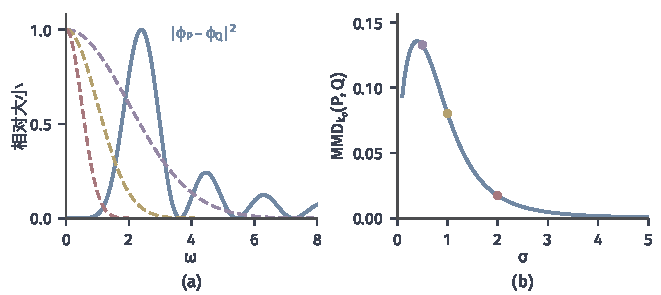
\includegraphics[width=112mm]{figures/07-probability/04-distribution-analysis/matplotlib/dcomp-mmd-spectrum/figure.pdf}
 \caption{高斯核MMD的频率图景，$P=\mathcal{N}(0,1)$，$Q=\operatorname{Unif}(-\sqrt3,\sqrt3)$。(a)蓝线是$\lvert\phi_P(\omega)-\phi_Q(\omega)\rvert^{2}$（除以最大值约$0.0679$）；虚线是频率权重$\exp(-\sigma^{2}\omega^{2}/2)$，紫、黄、红依次为$\sigma=0.5,1,2$。(b)$\operatorname{MMD}_{k_\sigma}(P,Q)$随$\sigma$的变化，三个点对应(a)中的三个带宽，数值约为$0.1329$，$0.0804$，$0.0174$。}
 \label{fig:dcomp-mmd-spectrum}
\end{BookInlineFigure}

特征核只保证“零值等价于分布相同”。一列分布的MMD趋于零能否推出弱收敛，是另一个问题，第~\ref{sec:dcomp-mmd-convergence}节专门讨论。

\section{Wasserstein距离}
\label{sec:dcomp-wasserstein}

回到章首的两个单点分布$\delta_0$与$\delta_h$。总变差是$1$，Hellinger距离是$1$，KL散度是$+\infty$，这些量都认为两者“完全不同”，无论$h$多小。它们只比较同一位置上的概率，不知道$0$与$h$离得很近。若取值空间有距离，可以换一种问法：把一个分布的概率质量搬成另一个分布的样子，最少要花多大力气？把概率质量想成一堆土，搬一份土的成本是质量乘以搬运距离，$\delta_0$变成$\delta_h$只需把全部质量搬动$h$，成本是$h$，随$h\to0$趋于零。本节把这个想法写成定义。

\subsection{耦合成本}
\label{sec:dcomp-coupling-cost}

搬运方案要说清每一份质量从哪里来、到哪里去。用概率的语言，就是一个二维分布$\pi(\mathrm{d}x,\mathrm{d}y)$：$\pi$在$(x,y)$附近的质量表示从$x$附近搬到$y$附近的土量。从$x$出发的总量必须是$P$在$x$处原有的量，到达$y$的总量必须是$Q$在$y$处需要的量，即$\pi$的两个边缘分别是$P$与$Q$。

\begin{definition}[耦合]
\label{def:dcomp-coupling}
设$\mu,\nu$分别是$\mathcal{X}$与$\mathcal{Y}$上的概率分布。若$\mathcal{X}\times\mathcal{Y}$上的概率分布$\pi$满足
\begin{equation}
 \pi(A\times\mathcal{Y})=\mu(A),\qquad\pi(\mathcal{X}\times B)=\nu(B)
 \label{eq:dcomp-coupling-marginals}
\end{equation}
对一切可测集$A,B$成立，则称$\pi$为$\mu$与$\nu$的一个\term{耦合}（coupling）。全体耦合记作$\Pi(\mu,\nu)$。
\end{definition}

等价地说，耦合是一对定义在同一概率空间上的随机变量$(X,Y)$的联合分布，$X\sim\mu$，$Y\sim\nu$。耦合总是存在，例如乘积分布$\mu\otimes\nu$，它对应让$X$与$Y$独立。耦合只约束边缘，联合分布本身有很大的选择余地。本节按度量空间上测度的习惯，把两个分布记作$\mu,\nu$；需要与前面的量并列比较时仍写$P,Q$。

距离需要底层空间的几何结构。设$(E,d)$是度量空间，并且完备、可分，这样的空间称为\term{Polish空间}（Polish space）。$\mathbb{R}^{d}$、它的闭子集、可数离散集都是Polish空间。完备可分保证了耦合与最优耦合理论中需要的紧性和可测性，度量空间的基本概念可参考\BookChapterRef{chap:metric-spaces}{卷四第2章“度量空间”}。对$1\leq p<\infty$，记$\mathcal{P}_p(E)$为满足
\begin{equation}
 \int_{E}d(x,x_0)^{p}\,\mu(\mathrm{d}x)<\infty
 \label{eq:dcomp-p-moment}
\end{equation}
的概率分布全体，其中$x_0\in E$是任取的基点；由$d(x,x_1)\leq d(x,x_0)+d(x_0,x_1)$，换一个基点不改变有限性。

\begin{definition}[Wasserstein距离]
\label{def:dcomp-wasserstein}
设$(E,d)$是Polish空间，$1\leq p<\infty$，$\mu,\nu\in\mathcal{P}_p(E)$。称
\begin{equation}
 W_p(\mu,\nu)=\Bigl(\inf_{\pi\in\Pi(\mu,\nu)}\int_{E\times E}d(x,y)^{p}\,\pi(\mathrm{d}x,\mathrm{d}y)\Bigr)^{1/p}
 \label{eq:dcomp-wasserstein-def}
\end{equation}
为$\mu$与$\nu$之间的$p$阶\term{Wasserstein距离}（Wasserstein distance）。
\end{definition}

有限矩条件保证下确界有限。用独立耦合，再用$(a+b)^{p}\leq2^{p-1}(a^{p}+b^{p})$与$d(x,y)\leq d(x,x_0)+d(x_0,y)$，
\[
 \begin{aligned}
 &\int d(x,y)^{p}\,(\mu\otimes\nu)(\mathrm{d}x,\mathrm{d}y)\\
 &\qquad\leq2^{p-1}\Bigl(\int d(x,x_0)^{p}\,\mu(\mathrm{d}x)+\int d(x_0,y)^{p}\,\nu(\mathrm{d}y)\Bigr)<\infty .
 \end{aligned}
\]
$W_p$是$\mathcal{P}_p(E)$上的距离。对称与非负直接来自定义；$W_p(\mu,\nu)=0$推出$\mu=\nu$，要用到下确界可以被某个耦合达到；三角不等式要把$\mu$到$\nu$与$\nu$到$\rho$的两个耦合沿公共边缘$\nu$粘合成一个三维分布，用到第~\ref{chap:conditional-distributions}章的正则条件分布。这两步的证明较长，读者可查阅~\scite{math-villani2009transport}。怎样求出最优耦合以及相应的算法由第~\ref{chap:optimal-transport}章研究。

\paragraph{单点分布}
$\delta_x$与$\delta_y$的耦合只有一个：两个边缘都是单点，联合分布只能是$\delta_{(x,y)}$。于是
\[
 W_p(\delta_x,\delta_y)=d(x,y) .
\]
图~\ref{fig:dcomp-point-shift}把它与前面的比较量放在一起：随着平移量$h$变小，$W_p=h$连续地趋于零，总变差与Hellinger距离却一直停在$1$。高斯核MMD介于两者之间：$h$小时它约等于$h$，$h$大时趋于$\sqrt2$，因为核只能“看见”带宽范围内的距离。

\begin{BookInlineFigure}
 \centering
 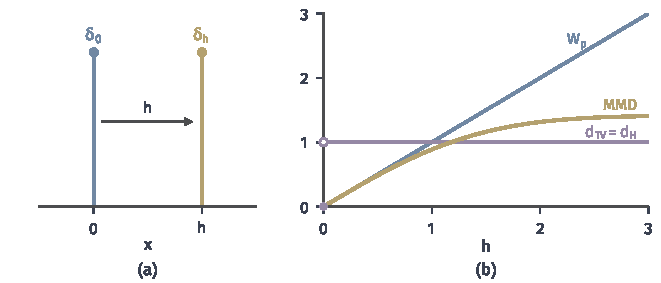
\includegraphics[width=112mm]{figures/07-probability/04-distribution-analysis/matplotlib/dcomp-point-shift/figure.pdf}
 \caption{单点分布的平移。(a)$\delta_0$与$\delta_h$。(b)作为$h$的函数：$W_p=h$（蓝，对所有$p$相同），$d_{\mathrm{TV}}=d_{\mathrm{H}}=1$（紫，$h=0$时为$0$），$\sigma=1$高斯核的$\operatorname{MMD}=\sqrt{2-2\mathrm{e}^{-h^{2}/2}}$（黄）。KL散度对每个$h>0$都是$+\infty$。}
 \label{fig:dcomp-point-shift}
\end{BookInlineFigure}

\paragraph{例表上的搬运}
把例表的三个取值看成实数轴上的位置$0,1,2$，距离取$\lvert x-y\rvert$。耦合是一个$3\times3$的非负矩阵$\bm{\pi}$，行和为$\bm{p}=(0.6,0.3,0.1)$，列和为$\bm{q}=(0.3,0.3,0.4)$，成本是$\sum_{i,j}\bm{\pi}_{i,j}\lvert i-j\rvert^{p}$（下标从$0$起）。图~\ref{fig:dcomp-coupling-plans}给出三个耦合。

\begin{BookInlineFigure}
 \centering
 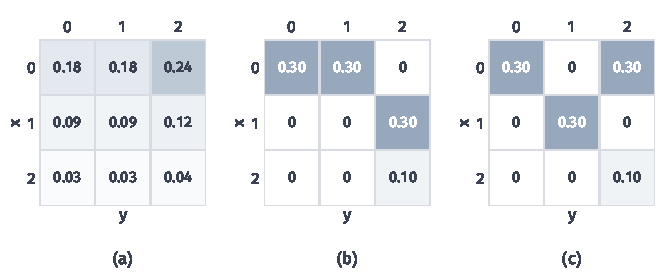
\includegraphics[width=112mm]{figures/07-probability/04-distribution-analysis/matplotlib/dcomp-coupling-plans/figure.pdf}
 \caption{例表的三个耦合，行是$x$（$P$），列是$y$（$Q$），颜色越深质量越大。(a)独立耦合$\bm{p}\bm{q}^{\top}$：$\sum\bm{\pi}_{i,j}\lvert i-j\rvert=0.96$，$\sum\bm{\pi}_{i,j}\lvert i-j\rvert^{2}=1.5$。(b)逐格搬运：两项成本都是$0.6$。(c)跳格搬运：一阶成本$0.6$，二阶成本$1.2$。}
 \label{fig:dcomp-coupling-plans}
\end{BookInlineFigure}

独立耦合让每一份质量都随机地去往目的地，许多质量被不必要地搬远，一阶成本是$0.96$。逐格搬运把点$0$多出的$0.3$搬到点$1$，再把点$1$原有的$0.3$搬到点$2$；跳格搬运直接把$0.3$从$0$搬到$2$，点$1$不动，见图~\ref{fig:dcomp-transport-arrows}。两种方案的一阶成本都是$0.6$。

\begin{BookInlineFigure}
 \centering
 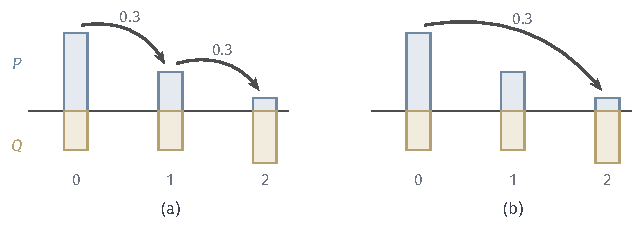
\includegraphics[width=108mm]{figures/07-probability/04-distribution-analysis/tikz/dcomp-transport-arrows/figure.pdf}
 \caption{例表的两种搬运方案，蓝柱向上是$P$，黄柱向下是$Q$，箭头上的数是搬运的质量。(a)逐格搬运：$0\to1$与$1\to2$各$0.3$。(b)跳格搬运：$0\to2$搬$0.3$。}
 \label{fig:dcomp-transport-arrows}
\end{BookInlineFigure}

$0.6$已经是最小值。对任何耦合$(X,Y)$，期望的绝对值不超过绝对值的期望，所以
\[
 \mathbb{E}\lvert X-Y\rvert\geq\lvert\mathbb{E}[X]-\mathbb{E}[Y]\rvert=\lvert0.5-1.1\rvert=0.6 ,
\]
所以$W_1(P,Q)=0.6$，两个方案都最优。二阶成本把两者分开了。记$a=\bm{\pi}_{0,1}$，$b=\bm{\pi}_{0,2}$，$c=\bm{\pi}_{1,2}$。点$0$只能留下$0.3$，所以至少$0.3$离开它，$a+b\geq0.3$；点$2$原有的$0.1$至多满足它的需要$0.4$中的$0.1$，所以$b+c\geq0.3$。成本矩阵中其余元素非负，于是
\[
 \sum_{i,j}\bm{\pi}_{i,j}\lvert i-j\rvert^{2}\geq a+4b+c=(a+b)+(b+c)+2b\geq0.6 ,
\]
等号要求$b=0$，$a=c=0.3$，正是逐格搬运。所以$W_2(P,Q)=\sqrt{0.6}\approx0.7746$。$p=1$时成本按距离线性计，一次跳两格与两次各跳一格花费相同；$p>1$时长距离被加倍惩罚，最优方案倾向于让每份质量只走短路。

这个例子也说明了定义中的“下确界”不能省略。如果$X,Y$已经由某个实验在同一概率空间上给出，它们的联合分布只是$\Pi(P,Q)$中的一个元素，$\mathbb{E}\lvert X-Y\rvert^{p}$通常大于$W_p^{p}$。Wasserstein距离只依赖两个边缘分布，与它们碰巧以怎样的方式一起出现无关。第~\ref{sec:dcomp-wasserstein-convergence}节会再回到这一点。

\paragraph{离散度量下的总变差}
在任意集合上取离散度量$d(x,y)=\mathbf{1}_{\{x\neq y\}}$，搬运成本只问“动没动”，不问距离。这时$W_1$正是总变差：
\begin{equation}
 \inf_{\pi\in\Pi(P,Q)}\pi\bigl(\{(x,y):x\neq y\}\bigr)=d_{\mathrm{TV}}(P,Q) .
 \label{eq:dcomp-maximal-coupling}
\end{equation}
一方面，对任何耦合$(X,Y)$与事件$A$，
\[
 P(A)-Q(A)=\mathbb{P}(X\in A)-\mathbb{P}(Y\in A)\leq\mathbb{P}(X\in A,\,Y\notin A)\leq\mathbb{P}(X\neq Y),
\]
所以左边不小于$d_{\mathrm{TV}}$。另一方面可以构造达到它的耦合。记$\delta=d_{\mathrm{TV}}(P,Q)$，设$0<\delta<1$（$\delta=0$时取$X=Y$，$\delta=1$时任何耦合都满足$\mathbb{P}(X\neq Y)\leq1$）。以概率$1-\delta$令$X=Y$，按密度$\min(p,q)/(1-\delta)$抽取；以概率$\delta$让$X$按密度$(p-q)^{+}/\delta$、$Y$按密度$(q-p)^{+}/\delta$独立抽取。由式~\eqref{eq:dcomp-tv-density}，这些都是概率密度。$X$的密度是$\min(p,q)+(p-q)^{+}=p$，$Y$的密度同理是$q$；第二种情形下$X$落在$\{p>q\}$而$Y$落在$\{q>p\}$，必然不等，所以$\mathbb{P}(X\neq Y)=\delta$。这样的耦合称为\term{最大耦合}（maximal coupling），它让两个变量以尽可能大的概率相等。总变差因此有了一个搬运解释：两个分布重叠的那部分质量原地不动，剩下的$d_{\mathrm{TV}}$那部分必须挪走。

\subsection{一阶距离的函数表示}
\label{sec:dcomp-kr}

例表上，$W_1$的下界来自函数$g(x)=x$的期望差。这不是巧合。若$g$是1-Lipschitz函数，即$\lvert g(x)-g(y)\rvert\leq d(x,y)$，则对任何耦合$(X,Y)$，
\[
 \mathbb{E}_{\mu}[g]-\mathbb{E}_{\nu}[g]=\mathbb{E}\bigl[g(X)-g(Y)\bigr]\leq\mathbb{E}\bigl[d(X,Y)\bigr] .
\]
对耦合取下确界，左边不超过$W_1(\mu,\nu)$。$g$的期望存在，因为$\lvert g(x)\rvert\leq\lvert g(x_0)\rvert+d(x,x_0)$，由一阶矩有限可积。所以每个1-Lipschitz函数都给出$W_1$的一个下界，而每个耦合都给出一个上界。两者在最优处相遇。

\begin{theorem}[Kantorovich--Rubinstein对偶]
\label{thm:dcomp-kantorovich-rubinstein}
设$(E,d)$是Polish空间，$\mu,\nu\in\mathcal{P}_1(E)$。则
\begin{equation}
 W_1(\mu,\nu)=\sup\Bigl\{\mathbb{E}_{\mu}[g]-\mathbb{E}_{\nu}[g]:\ \lvert g(x)-g(y)\rvert\leq d(x,y)\ \text{对一切}\ x,y\Bigr\} .
 \label{eq:dcomp-kr}
\end{equation}
\end{theorem}

上面已经证明了“$\geq$”。下面对两个分布都只有有限个支撑点的情形证明等号，一般情形的证明需要用有限支撑分布逼近并控制紧性，读者可查阅~\scite{math-villani2009transport}。这一结论称为\term{Kantorovich--Rubinstein对偶}（Kantorovich--Rubinstein duality）。

\begin{proof}[有限支撑情形的证明]
设$\mu=\sum_{i=1}^{m}a_i\delta_{x_i}$，$\nu=\sum_{j=1}^{n}b_j\delta_{y_j}$，记$c_{i,j}=d(x_i,y_j)$。两个边缘分别集中在$\{x_i\}$与$\{y_j\}$上，所以耦合集中在这些点对上，由矩阵$\bm{\pi}_{i,j}$描述。$W_1$是线性规划
\[
 \min_{\bm{\pi}\geq\bm{0}}\ \sum_{i,j}c_{i,j}\bm{\pi}_{i,j}\quad\text{s.t.}\quad\sum_{j}\bm{\pi}_{i,j}=a_i,\quad\sum_{i}\bm{\pi}_{i,j}=b_j
\]
的最优值。它的对偶问题是在约束$u_i+v_j\leq c_{i,j}$下最大化$\sum_ia_iu_i+\sum_jb_jv_j$。原问题可行（独立耦合）且目标有下界$0$，由线性规划的强对偶定理，对偶问题有最优解$(\bm{u},\bm{v})$，最优值等于$W_1$，可参考\BookChapterRef{chap:linear-programming}{卷五第2章“线性规划”}。

用对偶解构造一个函数：
\[
 g(z)=\min_{1\leq j\leq n}\bigl(d(z,y_j)-v_j\bigr),\qquad z\in E .
\]
每个$z\mapsto d(z,y_j)-v_j$都是1-Lipschitz函数，有限个1-Lipschitz函数的最小值仍是1-Lipschitz函数。由对偶约束，$u_i\leq c_{i,j}-v_j$对每个$j$成立，所以$g(x_i)\geq u_i$；取$z=y_j$并只看第$j$项，得$g(y_j)\leq-v_j$。于是
\[
 \mathbb{E}_{\mu}[g]-\mathbb{E}_{\nu}[g]=\sum_ia_ig(x_i)-\sum_jb_jg(y_j)\geq\sum_ia_iu_i+\sum_jb_jv_j=W_1(\mu,\nu) .
\]
与已经证明的“$\leq$”合起来，$g$达到了式~\eqref{eq:dcomp-kr}的上确界。
\end{proof}

证明中的$g$由一族“锥形”函数取下包络得到，每个锥以某个$y_j$为顶点、坡度为$1$、整体下移$v_j$。在例表上，$\mu=P$，$\nu=Q$，一个对偶最优解是$\bm{u}=(0,-1,-2)$，$\bm{v}=(0,1,2)$：约束$u_i+v_j=j-i\leq\lvert i-j\rvert$成立，目标值$-0.5+1.1=0.6$。构造出的$g$在$[0,2]$上就是$g(z)=-z$，见图~\ref{fig:dcomp-kr-dual}(b)；它与例表上的下界只差一个符号，$\mathbb{E}_{P}[g]-\mathbb{E}_{Q}[g]=0.6$。图中(a)画出两个分布函数，它们之间的面积也是$0.6$。实数轴上$W_1$与这块面积之间的一般关系属于一维运输问题，在第~\ref{chap:optimal-transport}章讨论。

\begin{BookInlineFigure}
 \centering
 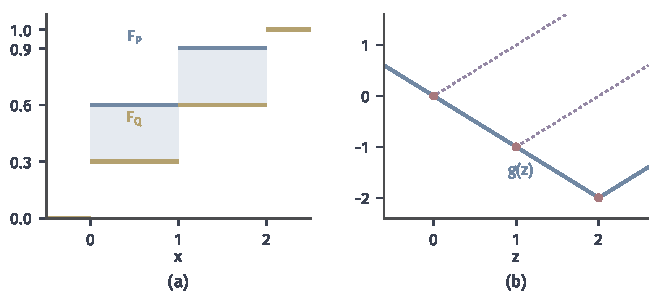
\includegraphics[width=112mm]{figures/07-probability/04-distribution-analysis/matplotlib/dcomp-kr-dual/figure.pdf}
 \caption{例表上的Kantorovich--Rubinstein对偶。(a)分布函数$F_P$（蓝）与$F_Q$（黄），两者之间浅蓝区域的面积为$0.6$。(b)紫色点线是三个锥$\lvert z-y_j\rvert-v_j$，$\bm{v}=(0,1,2)$；蓝线是它们的下包络$g$，红点是$g(x_i)=u_i$。}
 \label{fig:dcomp-kr-dual}
\end{BookInlineFigure}

式~\eqref{eq:dcomp-kr}把$W_1$放进了第~\ref{sec:dcomp-ipm}节的框架：它是由1-Lipschitz函数类生成的积分概率度量。与总变差的式~\eqref{eq:dcomp-tv-dual}对照，总变差的测试函数要求有界、允许跳跃；$W_1$的测试函数要求不能变化太快，但允许无界增长。前者对微小平移敏感，后者对远处的小质量敏感。

\paragraph{高阶距离不是积分概率度量}
$p>1$时，不能把式~\eqref{eq:dcomp-kr}中的$W_1$换成$W_p$，而且任何函数类都不行。原因是积分概率度量沿混合是线性的：对混合分布$\nu_\varepsilon=(1-\varepsilon)\mu+\varepsilon\nu$，每个$g$满足
\[
 \mathbb{E}_{\nu_\varepsilon}[g]-\mathbb{E}_{\mu}[g]=\varepsilon\bigl(\mathbb{E}_{\nu}[g]-\mathbb{E}_{\mu}[g]\bigr),
\]
取上确界得
\[
 d_{\mathcal{G}}(\mu,\nu_\varepsilon)=\varepsilon\,d_{\mathcal{G}}(\mu,\nu) .
\]
取$\mu=\delta_0$与$\nu=\delta_1$，混合分布把$\varepsilon$的质量放在$1$处。最优耦合让$1-\varepsilon$的质量留在原地，把$\varepsilon$的质量搬动距离$1$，所以
\[
 W_p(\mu,\nu_\varepsilon)=\varepsilon^{1/p} .
\]
$p=1$时它是$\varepsilon$，与线性相容；$p=2$时是$\sqrt\varepsilon$，见图~\ref{fig:dcomp-wp-mixture}。若$W_2=d_{\mathcal{G}}$对某个函数类成立，就会有$\sqrt\varepsilon=\varepsilon\cdot1$对一切$\varepsilon\in(0,1)$成立，矛盾。$W_p$对“少量质量走很远”的惩罚是非线性的，这是$p$次方成本带来的。

\begin{BookInlineFigure}
 \centering
 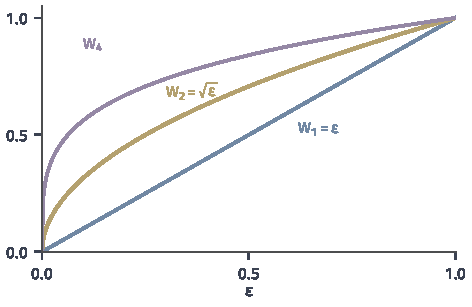
\includegraphics[width=80mm]{figures/07-probability/04-distribution-analysis/matplotlib/dcomp-wp-mixture/figure.pdf}
 \caption{$\delta_0$与$(1-\varepsilon)\delta_0+\varepsilon\delta_1$之间的$W_p=\varepsilon^{1/p}$：$p=1$（蓝），$p=2$（黄），$p=4$（紫）。任何积分概率度量沿这条混合线段都是$\varepsilon$的线性函数，只有$p=1$相容。}
 \label{fig:dcomp-wp-mixture}
\end{BookInlineFigure}

\section{期望误差}
\label{sec:dcomp-expectation}

比较分布往往是为了一个具体目的：用$Q$代替$P$计算某个平均$\mathbb{E}_{P}[g]$，误差有多大？前面几节已经分别得到有界函数、Lipschitz函数与RKHS函数的期望差表示。把这些结果放在一起，问题就变成：给定的$g$属于哪一类，范数是多少，该用哪个比较量。无界的$g$不属于这些类中的某几个，需要另外控制尾部；KL散度不是积分概率度量，要借助指数矩才能控制期望。

\subsection{函数范围内的误差}
\label{sec:dcomp-function-bounds}

把式~\eqref{eq:dcomp-tv-osc}、式~\eqref{eq:dcomp-kr}与式~\eqref{eq:dcomp-mmd-def}中的函数类按范数缩放，就得到三个上界。

\begin{theorem}[三类函数的期望差]
\label{thm:dcomp-three-bounds}
设$P,Q$是同一空间上的概率分布。
\begin{enumerate}
 \item 若$g$可测且有界，则期望差的绝对值不超过$\operatorname{osc}(g)\,d_{\mathrm{TV}}(P,Q)$。
 \item 若空间是Polish空间，$P,Q\in\mathcal{P}_1$，$g$是Lipschitz函数，常数为$\operatorname{Lip}(g)$，则
 \begin{equation}
  \bigl\lvert\mathbb{E}_{P}[g]-\mathbb{E}_{Q}[g]\bigr\rvert\leq\operatorname{Lip}(g)\,W_1(P,Q) .
  \label{eq:dcomp-lip-bound}
 \end{equation}
 \item 若$k$满足定理~\ref{thm:dcomp-kernel-mean}的条件，$P,Q$满足式~\eqref{eq:dcomp-kernel-moment}，$g\in\mathcal{H}$，则
 \begin{equation}
  \bigl\lvert\mathbb{E}_{P}[g]-\mathbb{E}_{Q}[g]\bigr\rvert\leq\lVert g\rVert_{\mathcal{H}}\operatorname{MMD}_k(P,Q) .
  \label{eq:dcomp-rkhs-bound}
 \end{equation}
\end{enumerate}
\end{theorem}

\begin{proof}
第一条即式~\eqref{eq:dcomp-tv-osc}。第二条：$\operatorname{Lip}(g)=0$时$g$为常数，两边为零；否则$g/\operatorname{Lip}(g)$是1-Lipschitz函数，由式~\eqref{eq:dcomp-kr}得结论，$g$在$P,Q$下可积已在第~\ref{sec:dcomp-kr}节说明。第三条：$g=0$时两边为零；否则$g/\lVert g\rVert_{\mathcal{H}}$在单位球中，由式~\eqref{eq:dcomp-mmd-def}得结论。
\end{proof}

定理的三条要求不同的东西，选择哪一条取决于$g$的性质。示性函数$\mathbf{1}_{A}$有界，但有跳跃，不是Lipschitz函数，也不在高斯核的RKHS中（该空间中的函数都连续），只能用总变差。$g(x)=x$是1-Lipschitz函数，但无界；高斯核有界，由定理~\ref{thm:dcomp-kernel-mean}证明中的估计，$\lvert g(x)\rvert$不超过$\lVert g\rVert_{\mathcal{H}}\sqrt{k(x,x)}$，而高斯核的$k(x,x)=1$，所以它的RKHS只含有界函数，所以只能用$W_1$。光滑、有界的函数三条都可以用，这时要比较哪个上界更小。

\paragraph{同一个函数的三个上界}
取$P=\delta_0$，$Q=\delta_h$，$g(x)=\exp(-x^{2}/2)$，它是$\sigma=1$高斯核的截面$k(0,\cdot)$。由式~\eqref{eq:dcomp-reproducing}，$\lVert g\rVert_{\mathcal{H}}=\sqrt{k(0,0)}=1$；它的振幅为$1$；导数$-x\mathrm{e}^{-x^{2}/2}$的绝对值在$x=\pm1$处最大，Lipschitz常数是$\mathrm{e}^{-1/2}\approx0.6065$。真实的误差和三个上界分别是
\[
 1-\mathrm{e}^{-h^{2}/2},\qquad 1,\qquad\mathrm{e}^{-1/2}h,\qquad\sqrt{2-2\mathrm{e}^{-h^{2}/2}} .
\]
$h=0.5$时，真实误差约为$0.1175$，$W_1$上界约为$0.3033$，MMD上界约为$0.4848$，总变差上界是$1$。图~\ref{fig:dcomp-three-bounds}显示，小平移时$W_1$的界最紧，大平移时总变差的界最紧（误差本来就不会超过振幅），MMD的界在两者之间过渡。没有哪一个比较量对所有情形都最好。

\begin{BookInlineFigure}
 \centering
 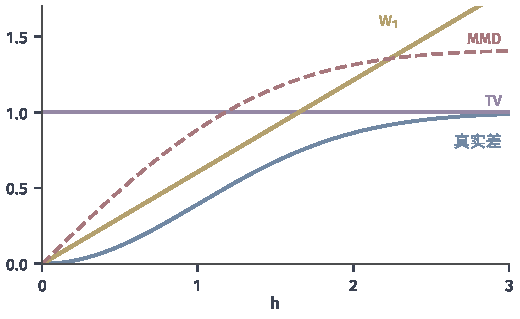
\includegraphics[width=88mm]{figures/07-probability/04-distribution-analysis/matplotlib/dcomp-three-bounds/figure.pdf}
 \caption{$P=\delta_0$，$Q=\delta_h$，$g(x)=\mathrm{e}^{-x^{2}/2}$时的期望误差。蓝线是真实误差$1-\mathrm{e}^{-h^{2}/2}$；紫线是总变差上界$\operatorname{osc}(g)\,d_{\mathrm{TV}}=1$，黄线是$W_1$上界$\mathrm{e}^{-1/2}h$，红色虚线是MMD上界$\sqrt{2-2\mathrm{e}^{-h^{2}/2}}$。}
 \label{fig:dcomp-three-bounds}
\end{BookInlineFigure}

\subsection{无界函数的尾部控制}
\label{sec:dcomp-tail}

许多需要计算的平均来自无界函数：均值、方差、多项式损失。分布在总变差或MMD意义下接近，只说明大部分质量摆放得差不多；极少的质量若落在很远的地方，无界函数会把它放大。下面先给出一个把问题拆开的不等式，再看反例。

\begin{lemma}[截断分解]
\label{lem:dcomp-truncation}
设$g$在$P,Q$下可积，$r>0$。记$g_r$为$g$在水平$r$处的截断，即把大于$r$的值改为$r$，小于$-r$的值改为$-r$。则
\begin{equation}
 \begin{aligned}
 \bigl\lvert\mathbb{E}_{P}[g]-\mathbb{E}_{Q}[g]\bigr\rvert&\leq\bigl\lvert\mathbb{E}_{P}[g_r]-\mathbb{E}_{Q}[g_r]\bigr\rvert\\
 &\quad+\mathbb{E}_{P}\bigl[\lvert g\rvert\mathbf{1}_{\{\lvert g\rvert>r\}}\bigr]+\mathbb{E}_{Q}\bigl[\lvert g\rvert\mathbf{1}_{\{\lvert g\rvert>r\}}\bigr] .
 \end{aligned}
 \label{eq:dcomp-truncation}
\end{equation}
\end{lemma}

\begin{proof}
$g-g_r$只在$\{\lvert g\rvert>r\}$上非零，那里$g-g_r$的绝对值是$\lvert g\rvert-r$，不超过$\lvert g\rvert$，所以
\[
 \bigl\lvert\mathbb{E}_{P}[g-g_r]\bigr\rvert\leq\mathbb{E}_{P}\bigl[\lvert g\rvert\mathbf{1}_{\{\lvert g\rvert>r\}}\bigr],
\]
对$Q$同理。把$g=g_r+(g-g_r)$代入期望差，用三角不等式即得。
\end{proof}

右边第一项是有界函数的期望差，可用前面的比较量控制，例如不超过$2r\,d_{\mathrm{TV}}(P,Q)$；若$g$是Lipschitz函数，$g_r$也是，并且常数不变，可以用$W_1$。后两项是两个分布各自的尾部，比较量对它们无能为力，必须由矩条件单独控制。对一列分布，需要的就是尾部的一致小。

\begin{theorem}[一致可积时期望收敛]
\label{thm:dcomp-ui-convergence}
设$d_{\mathrm{TV}}(P_n,P)\to0$，$g$在每个$P_n$与$P$下可积，并且
\begin{equation}
 \lim_{r\to\infty}\sup_{n}\mathbb{E}_{P_n}\bigl[\lvert g\rvert\mathbf{1}_{\{\lvert g\rvert>r\}}\bigr]=0 .
 \label{eq:dcomp-ui}
\end{equation}
则$\mathbb{E}_{P_n}[g]\to\mathbb{E}_{P}[g]$。
\end{theorem}

\begin{proof}
任给$\varepsilon>0$。由式~\eqref{eq:dcomp-ui}与$\mathbb{E}_{P}\lvert g\rvert<\infty$，可以取$r$，使式~\eqref{eq:dcomp-truncation}的两个尾部项对每个$P_n$与$P$都小于$\varepsilon$。由式~\eqref{eq:dcomp-truncation}与$\operatorname{osc}(g_r)\leq2r$，
\[
 \bigl\lvert\mathbb{E}_{P_n}[g]-\mathbb{E}_{P}[g]\bigr\rvert\leq2r\,d_{\mathrm{TV}}(P_n,P)+2\varepsilon .
\]
固定$r$令$n\to\infty$，上极限不超过$2\varepsilon$；$\varepsilon$任意，结论成立。
\end{proof}

条件~\eqref{eq:dcomp-ui}正是第~\ref{chap:random-variable-convergence}章的一致可积。多项式增长的函数可以用高一点的矩保证它。设$\lvert g(x)\rvert\leq C(1+\lvert x\rvert^{k})$，并且对某个$\delta>0$，各$P_n$的$k+\delta$阶绝对矩一致地不超过$M$。记$q=1+\delta/k$。在$\{\lvert g\rvert>r\}$上，$\lvert g\rvert\leq\lvert g\rvert^{q}/r^{q-1}$，又由$(a+b)^{q}\leq2^{q-1}(a^{q}+b^{q})$，
\[
 \mathbb{E}_{P_n}\bigl[\lvert g\rvert\mathbf{1}_{\{\lvert g\rvert>r\}}\bigr]\leq\frac{\mathbb{E}_{P_n}\lvert g\rvert^{q}}{r^{q-1}}\leq\frac{C^{q}2^{q-1}(1+M)}{r^{\delta/k}},
\]
关于$n$一致地趋于零。只有$k$阶矩有界是不够的，下面的例子说明这一点。

\paragraph{远处的小质量}
令$P_n=(1-\tfrac1n)\delta_0+\tfrac1n\delta_n$，与$\delta_0$比较。总变差是$1/n$，高斯核MMD约为$\sqrt2/n$，都趋于零。每个$P_n$只有两个支撑点，各阶矩都有限。可是均值与二阶矩是
\[
 \mathbb{E}_{P_n}[X]=\frac1n\cdot n=1,\qquad\mathbb{E}_{P_n}[X^{2}]=\frac1n\cdot n^{2}=n,
\]
不收敛到$\delta_0$下的$0$。尾部条件~\eqref{eq:dcomp-ui}对$g(x)=x$不成立：$n>r$时$\mathbb{E}_{P_n}[X\mathbf{1}_{\{X>r\}}]=1$。逐个分布的矩有限，不能代替一致的尾部控制。

$W_1$能看见这一份远处的质量：把$1/n$的质量从$n$搬回$0$，成本是$1$，所以$W_1(P_n,\delta_0)=1$，与均值的差一致，这正是式~\eqref{eq:dcomp-lip-bound}对$g(x)=x$的含义。但$W_1$也有看不见的东西。令
\[
 R_n=(1-n^{-2})\delta_0+n^{-2}\delta_n .
\]
把$n^{-2}$的质量搬动距离$n$，一阶与二阶的搬运成本分别给出
\[
 W_1(R_n,\delta_0)=\frac1n\to0,\qquad W_2(R_n,\delta_0)=\bigl(n^{-2}\cdot n^{2}\bigr)^{1/2}=1 ,
\]
而$R_n$的二阶矩恒为$1$，不趋于零。图~\ref{fig:dcomp-far-mass}画出这两族分布。控制$k$阶增长的函数，要用$k$阶的比较量或额外的一致可积条件。

\begin{BookInlineFigure}
 \centering
 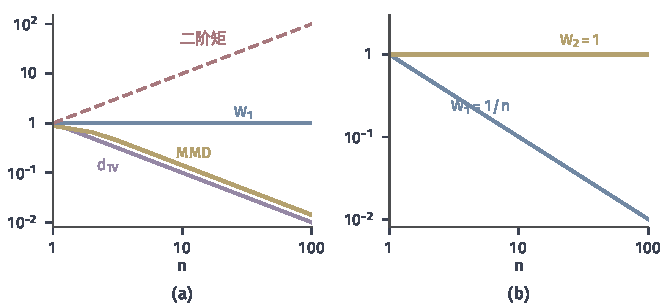
\includegraphics[width=112mm]{figures/07-probability/04-distribution-analysis/matplotlib/dcomp-far-mass/figure.pdf}
 \caption{远处的小质量，与$\delta_0$比较，双对数坐标。(a)$P_n=(1-\tfrac1n)\delta_0+\tfrac1n\delta_n$：$d_{\mathrm{TV}}=1/n$（紫），$\sigma=1$高斯核MMD（黄），$W_1=1$（蓝），二阶矩$n$（红色虚线）。(b)$R_n=(1-n^{-2})\delta_0+n^{-2}\delta_n$：$W_1=1/n$（蓝），$W_2=1$（黄）。}
 \label{fig:dcomp-far-mass}
\end{BookInlineFigure}

\subsection{KL与指数矩}
\label{sec:dcomp-kl-exp}

KL散度没有写成积分概率度量的形式，它能控制期望吗？先看有界函数：第~\ref{sec:dcomp-pinsker}节将证明KL散度控制总变差，于是它也控制有界函数的期望差。对无界函数，KL散度单独不够，还需要参考分布$Q$下的指数矩。关键工具是把$Q$按$\mathrm{e}^{g}$重新加权。

设$g$可测，$Z=\mathbb{E}_{Q}[\mathrm{e}^{g}]<\infty$。定义新的分布$Q_g$，
\begin{equation}
 \frac{\mathrm{d}Q_g}{\mathrm{d}Q}=\frac{\mathrm{e}^{g}}{Z} .
 \label{eq:dcomp-tilt}
\end{equation}
它把$Q$的质量向$g$大的地方倾斜，称为\term{指数倾斜}（exponential tilting）。密度$\mathrm{e}^{g}/Z$处处为正，所以$Q$与$Q_g$互相绝对连续。

\begin{lemma}[KL与对数矩母函数]
\label{lem:dcomp-dv}
设$D_{\mathrm{KL}}(P\Vert Q)<\infty$，$\mathbb{E}_{Q}[\mathrm{e}^{g}]<\infty$，$\mathbb{E}_{P}\lvert g\rvert<\infty$。则
\begin{equation}
 \mathbb{E}_{P}[g]\leq D_{\mathrm{KL}}(P\Vert Q)+\ln\mathbb{E}_{Q}\bigl[\mathrm{e}^{g}\bigr] .
 \label{eq:dcomp-dv}
\end{equation}
\end{lemma}

\begin{proof}
$P\ll Q$，$Q\ll Q_g$，所以$P\ll Q_g$，并且由密度的链式法则与式~\eqref{eq:dcomp-tilt}，
\[
 \ln\frac{\mathrm{d}P}{\mathrm{d}Q_g}=\ln\frac{\mathrm{d}P}{\mathrm{d}Q}-g+\ln Z .
\]
$D_{\mathrm{KL}}(P\Vert Q)$有限且对数比的负部可积，所以$\ln(\mathrm{d}P/\mathrm{d}Q)$在$P$下可积；$g$也可积。对上式在$P$下逐项取期望，并用Gibbs不等式，
\[
 0\leq D_{\mathrm{KL}}(P\Vert Q_g)=D_{\mathrm{KL}}(P\Vert Q)-\mathbb{E}_{P}[g]+\ln Z .
\]
移项即得。
\end{proof}

不等式~\eqref{eq:dcomp-dv}只是把KL的非负性用在倾斜后的参考分布上。它的含义是：$P$相对$Q$偏离不大时，$g$在$P$下的平均不会远超“$Q$下的指数平均”。为了得到期望差，对$g$减去它在$Q$下的均值并乘以参数$\lambda$。

\begin{theorem}[KL控制的期望差]
\label{thm:dcomp-kl-expectation}
设$D_{\mathrm{KL}}(P\Vert Q)<\infty$，$g$在$P,Q$下可积，记
\begin{equation}
 \Lambda(\lambda)=\ln\mathbb{E}_{Q}\Bigl[\exp\bigl(\lambda(g-\mathbb{E}_{Q}[g])\bigr)\Bigr] .
 \label{eq:dcomp-centered-cgf}
\end{equation}
则对每个使$\Lambda(\lambda)$有限的$\lambda>0$，
\begin{equation}
 \begin{gathered}
 \mathbb{E}_{P}[g]-\mathbb{E}_{Q}[g]\leq\frac{D_{\mathrm{KL}}(P\Vert Q)+\Lambda(\lambda)}{\lambda},\\
 \mathbb{E}_{Q}[g]-\mathbb{E}_{P}[g]\leq\frac{D_{\mathrm{KL}}(P\Vert Q)+\Lambda(-\lambda)}{\lambda} .
 \end{gathered}
 \label{eq:dcomp-kl-two-sides}
\end{equation}
特别地，若对一切实数$\lambda$有$\Lambda(\lambda)\leq\lambda^{2}s^{2}/2$，则
\begin{equation}
 \bigl\lvert\mathbb{E}_{P}[g]-\mathbb{E}_{Q}[g]\bigr\rvert\leq\sqrt{2s^{2}D_{\mathrm{KL}}(P\Vert Q)} .
 \label{eq:dcomp-kl-subgaussian}
\end{equation}
\end{theorem}

\begin{proof}
把引理~\ref{lem:dcomp-dv}用于$\lambda(g-\mathbb{E}_{Q}[g])$，它在$P$下可积，在$Q$下的指数矩是$\mathrm{e}^{\Lambda(\lambda)}$：
\[
 \lambda\bigl(\mathbb{E}_{P}[g]-\mathbb{E}_{Q}[g]\bigr)\leq D_{\mathrm{KL}}(P\Vert Q)+\Lambda(\lambda) .
\]
除以$\lambda>0$得第一式。把同样的推理用于$-g$，它的中心化对数矩母函数是$\Lambda(-\lambda)$，得第二式。在次高斯条件下，两式右端都不超过$D/\lambda+\lambda s^{2}/2$（记$D=D_{\mathrm{KL}}(P\Vert Q)$）。$D>0$时取$\lambda=\sqrt{2D}/s$使它最小，最小值为$\sqrt{2s^{2}D}$；$D=0$时$P=Q$，两边都是零。
\end{proof}

\paragraph{高斯平移}
取$Q=\mathcal{N}(0,1)$与$g(x)=x$。中心化对数矩母函数是$\Lambda(\lambda)=\lambda^{2}/2$，次高斯条件以$s=1$成立。倾斜后的$Q_g$在$g=\lambda x$时是$\mathcal{N}(\lambda,1)$：$\mathrm{e}^{\lambda x}$乘以标准高斯密度，配方后正是均值为$\lambda$的高斯密度。再取$P$为均值$m$、方差$1$的高斯分布，由式~\eqref{eq:dcomp-kl-gauss}，KL散度是$m^{2}/2$，式~\eqref{eq:dcomp-kl-subgaussian}给出
\[
 \lvert\mathbb{E}_{P}[X]-\mathbb{E}_{Q}[X]\rvert\leq\sqrt{2\cdot m^{2}/2}=\lvert m\rvert ,
\]
等号成立，上界不能改进。若$P=\mathcal{N}(m,s'^{2})$，均值差仍是$m$，而KL散度多了方差失配的部分，上界变松；$m=1$时，$s'=\tfrac12$与$s'=2$的上界分别约为$1.279$与$1.617$。图~\ref{fig:dcomp-kl-tilt}画出倾斜后的分布与这些上界。

\begin{BookInlineFigure}
 \centering
 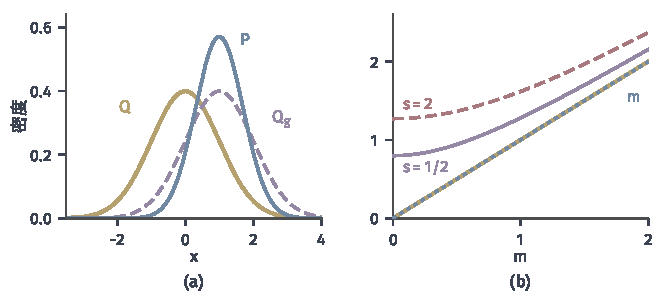
\includegraphics[width=112mm]{figures/07-probability/04-distribution-analysis/matplotlib/dcomp-kl-tilt/figure.pdf}
 \caption{KL散度与指数矩，$Q=\mathcal{N}(0,1)$，$g(x)=x$。(a)$Q$（黄），按$\mathrm{e}^{x}$倾斜后的$Q_g=\mathcal{N}(1,1)$（紫色虚线），以及$P=\mathcal{N}(1,0.7^{2})$（蓝）。(b)$P=\mathcal{N}(m,s'^{2})$时的真实均值差$m$（蓝色点线）与上界$\sqrt{2D_{\mathrm{KL}}(P\Vert Q)}$：$s'=1$（黄，与真实值重合），$s'=\tfrac12$（紫），$s'=2$（红色虚线）。}
 \label{fig:dcomp-kl-tilt}
\end{BookInlineFigure}

\paragraph{方向必须对应}
定理中的指数矩是在$Q$下计算的，而$Q$正是$D_{\mathrm{KL}}(P\Vert Q)$的第二个参数。只知道KL散度小、却不知道$Q$下的指数矩，期望可以相差无穷。在正整数上取
\[
 q_k=c\,k^{-3},\qquad r_k=\frac{6}{\pi^{2}}k^{-2},\qquad P_\varepsilon=(1-\varepsilon)Q+\varepsilon R ,
\]
其中$c\approx0.8319$。$Q$的均值是$c\sum_kk^{-2}\approx1.368$，有限，但它的尾部是多项式型的，$\mathbb{E}_{Q}[\mathrm{e}^{\lambda X}]$对任何$\lambda>0$都是无穷大。$R$的均值是$\tfrac{6}{\pi^{2}}\sum_kk^{-1}=+\infty$，所以$\mathbb{E}_{P_\varepsilon}[X]=+\infty$。另一方面，由$t\ln t$的凸性，
\[
 D_{\mathrm{KL}}(P_\varepsilon\Vert Q)=\mathbb{E}_{Q}\Bigl[f\Bigl((1-\varepsilon)+\varepsilon\frac{\mathrm{d}R}{\mathrm{d}Q}\Bigr)\Bigr]\leq(1-\varepsilon)f(1)+\varepsilon D_{\mathrm{KL}}(R\Vert Q),
\]
其中$f(t)=t\ln t$。而$D_{\mathrm{KL}}(R\Vert Q)=\sum_kr_k\ln(r_k/q_k)$中$\ln(r_k/q_k)$只按$\ln k$增长，级数收敛，数值约为$0.2563$。所以$P_\varepsilon$相对于$Q$的KL散度不超过$0.2563\,\varepsilon$，可以任意小，均值差却是无穷大。若指数矩只在$P$下有限，应当交换两个分布的角色，改用$D_{\mathrm{KL}}(Q\Vert P)$。

\section{比较量与收敛}
\label{sec:dcomp-convergence}

设$P_1,P_2,\dots$与$P$是一列分布，某个比较量$\rho(P_n,P)$趋于零。这能推出什么？能否推出另一个比较量也趋于零，能否推出第~\ref{chap:weak-convergence-of-distributions}章的弱收敛，矩是否也跟着收敛？本节逐一回答。弱收敛的定义与判别沿用那一章：$P_n\xrightarrow{\mathrm{w}}P$指对每个有界连续函数$f$，$\int f\,\mathrm{d}P_n\to\int f\,\mathrm{d}P$。那一章在$\mathbb{R}^{d}$上陈述；在一般度量空间上，定义只需把$\mathbb{R}^{d}$换成该空间，Portmanteau定理中“有界Lipschitz函数的期望收敛即可”这一判据的证明不变。

\subsection{散度与总变差的控制}
\label{sec:dcomp-pinsker}

先比较本身。总变差是最常用的标尺，KL散度和Hellinger距离与它有什么数量关系？本小节的对数一律取自然对数，总变差按定义~\ref{def:dcomp-tv}的约定，系数改变时下面的常数要相应改变。

\begin{theorem}[Pinsker不等式]
\label{thm:dcomp-pinsker}
对任意概率分布$P,Q$，
\begin{equation}
 d_{\mathrm{TV}}(P,Q)\leq\sqrt{\tfrac12D_{\mathrm{KL}}(P\Vert Q)} .
 \label{eq:dcomp-pinsker}
\end{equation}
\end{theorem}

\begin{proof}
\emph{化为两点分布。}若KL散度为$+\infty$，结论成立。设它有限，取$A^{*}=\{p>q\}$，用确定映射$x\mapsto\mathbf{1}_{A^{*}}(x)$把两个分布变成$\{0,1\}$上的两点分布$\operatorname{Bern}(a)$与$\operatorname{Bern}(b)$，其中$a=P(A^{*})$，$b=Q(A^{*})$。由定理~\ref{thm:dcomp-tv-density}，$d_{\mathrm{TV}}(P,Q)=a-b$；由定理~\ref{thm:dcomp-data-processing}，KL散度在映射后不增。所以只需证明两点分布的不等式
\[
 h(b)=a\ln\frac{a}{b}+(1-a)\ln\frac{1-a}{1-b}-2(a-b)^{2}\geq0,\qquad 0<b<1 .
\]

\emph{两点分布的情形。}固定$a\in[0,1]$，把$h$看成$b$的函数。$h(a)=0$。求导，
\[
 h'(b)=-\frac{a}{b}+\frac{1-a}{1-b}+4(a-b)=(b-a)\Bigl(\frac{1}{b(1-b)}-4\Bigr) .
\]
$b(1-b)\leq\tfrac14$，括号内非负，所以$h'(b)$与$b-a$同号：$h$在$b<a$时下降，在$b>a$时上升，最小值是$h(a)=0$。于是
\[
 D_{\mathrm{KL}}(P\Vert Q)\geq2(a-b)^{2}=2d_{\mathrm{TV}}^{2}(P,Q),
\]
开方即得。$b=0$或$1$而$a\neq b$时散度为$+\infty$，不需讨论。
\end{proof}

式~\eqref{eq:dcomp-pinsker}称为\term{Pinsker不等式}（Pinsker's inequality）。证明的思路值得留意：最坏事件$A^{*}$把一般分布压缩成一次是非判断，后处理不增加散度，于是一般情形归结为两点分布上的一元不等式。在例表上，$\sqrt{0.2773/2}\approx0.3723\geq0.3$。交换方向用$D_{\mathrm{KL}}(Q\Vert P)\approx0.3466$，得到$0.4163\geq0.3$，同样成立，因为总变差对称，任一方向的KL散度都控制它。图~\ref{fig:dcomp-pinsker}(a)在两点分布上比较两边：$P=\operatorname{Bern}(t)$，$Q=\operatorname{Bern}(\tfrac12)$，$t$接近$\tfrac12$时两条曲线几乎重合，常数$\tfrac12$不能再改进。

Pinsker不等式只有一个方向。总变差小不能推出KL散度小，甚至不能推出它有限。设$Q$在格点$0$处概率为零，例如$Q$是$\{1,2,\dots,10\}$上的均匀分布，令
\[
 P_\varepsilon=(1-\varepsilon)Q+\varepsilon\delta_0 .
\]
$P_\varepsilon$把$Q$的$\varepsilon$份质量挪到了点$0$，总变差是$\varepsilon$；但$P_\varepsilon(\{0\})=\varepsilon>0=Q(\{0\})$，$P_\varepsilon$不绝对连续于$Q$，$D_{\mathrm{KL}}(P_\varepsilon\Vert Q)=+\infty$。无论$\varepsilon$多小，总变差都看不出这个零概率格点上的冲突，KL散度则对它给出无穷大。

Hellinger距离与总变差之间是双向控制。

\begin{theorem}[Hellinger距离与总变差]
\label{thm:dcomp-hellinger-tv}
对任意概率分布$P,Q$，
\begin{equation}
 d_{\mathrm{H}}^{2}(P,Q)\leq d_{\mathrm{TV}}(P,Q)\leq d_{\mathrm{H}}(P,Q)\sqrt{2-d_{\mathrm{H}}^{2}(P,Q)} .
 \label{eq:dcomp-hellinger-tv}
\end{equation}
并且
\begin{equation}
 D_{\mathrm{KL}}(P\Vert Q)\geq2d_{\mathrm{H}}^{2}(P,Q) .
 \label{eq:dcomp-kl-hellinger}
\end{equation}
\end{theorem}

\begin{proof}
用共同支配测度写出密度。对每一点，
\[
 \lvert p-q\rvert=\lvert\sqrt{p}-\sqrt{q}\rvert\,(\sqrt{p}+\sqrt{q}),
\]
而右边第一个因子不超过第二个因子，所以$(\sqrt{p}-\sqrt{q})^{2}\leq\lvert p-q\rvert$。积分并乘以$\tfrac12$，得到左边的不等式。

对右边，用同一个分解与Cauchy--Schwarz不等式，
\[
 \frac12\int\lvert p-q\rvert\,\mathrm{d}\lambda\leq\frac12\Bigl(\int(\sqrt{p}-\sqrt{q})^{2}\,\mathrm{d}\lambda\Bigr)^{1/2}\Bigl(\int(\sqrt{p}+\sqrt{q})^{2}\,\mathrm{d}\lambda\Bigr)^{1/2} .
\]
第一个因子是$\sqrt2\,d_{\mathrm{H}}$；展开第二个因子中的平方，它是$(2+2B)^{1/2}$，由式~\eqref{eq:dcomp-hellinger-bc}，$B=1-d_{\mathrm{H}}^{2}$，所以第二个因子是$\sqrt2\,(2-d_{\mathrm{H}}^{2})^{1/2}$。代入即得右边的不等式。

最后，由定理~\ref{thm:dcomp-renyi-order}与式~\eqref{eq:dcomp-renyi-special}，$D_{\mathrm{KL}}\geq D_{1/2}=-2\ln B$，再由$-\ln B\geq1-B=d_{\mathrm{H}}^{2}$得式~\eqref{eq:dcomp-kl-hellinger}。
\end{proof}

在例表上，$d_{\mathrm{H}}^{2}\approx0.0757$，$d_{\mathrm{H}}\sqrt{2-d_{\mathrm{H}}^{2}}\approx0.3818$，总变差$0.3$确实夹在中间。式~\eqref{eq:dcomp-hellinger-tv}说明$d_{\mathrm{TV}}(P_n,P)\to0$当且仅当$d_{\mathrm{H}}(P_n,P)\to0$，两者定义的收敛相同，只是速度可能不同：一个是另一个的平方量级。图~\ref{fig:dcomp-pinsker}(b)在高斯平移族上画出这三条曲线以及Pinsker上界。

\begin{BookInlineFigure}
 \centering
 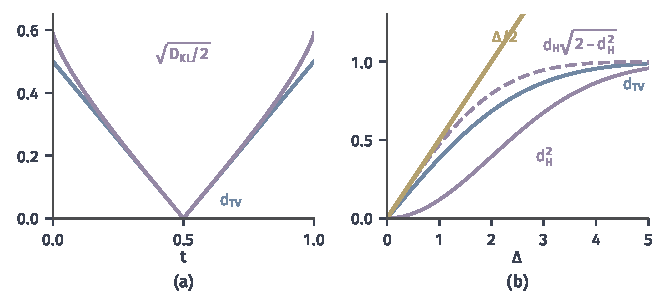
\includegraphics[width=112mm]{figures/07-probability/04-distribution-analysis/matplotlib/dcomp-pinsker/figure.pdf}
 \caption{散度对总变差的控制。(a)$P=\operatorname{Bern}(t)$，$Q=\operatorname{Bern}(\tfrac12)$：$d_{\mathrm{TV}}=\lvert t-\tfrac12\rvert$（蓝）与Pinsker上界$\sqrt{D_{\mathrm{KL}}(P\Vert Q)/2}$（紫）。(b)$P=\mathcal{N}(0,1)$，$Q=\mathcal{N}(\Delta,1)$：$d_{\mathrm{TV}}=2\Phi(\Delta/2)-1$（蓝），下界$d_{\mathrm{H}}^{2}=1-\mathrm{e}^{-\Delta^{2}/8}$（紫），上界$d_{\mathrm{H}}\sqrt{2-d_{\mathrm{H}}^{2}}$（紫色虚线），Pinsker上界$\Delta/2$（黄）。}
 \label{fig:dcomp-pinsker}
\end{BookInlineFigure}

\paragraph{总变差强于弱收敛}
若$d_{\mathrm{TV}}(P_n,P)\to0$，对每个有界连续$f$，由式~\eqref{eq:dcomp-tv-osc}，
\[
 \Bigl\lvert\int f\,\mathrm{d}P_n-\int f\,\mathrm{d}P\Bigr\rvert\leq2\lVert f\rVert_{\infty}\,d_{\mathrm{TV}}(P_n,P)\to0,
\]
所以$P_n\xrightarrow{\mathrm{w}}P$。反过来不成立。$\delta_{1/n}\xrightarrow{\mathrm{w}}\delta_0$，总变差却恒为$1$。一个更典型的例子是用离散分布逼近连续分布：令$U_n$是$n$个格点$(2k-1)/(2n)$（$k=1,\dots,n$）上的均匀分布，$U=\operatorname{Unif}(0,1)$。$U_n\xrightarrow{\mathrm{w}}U$，这是第~\ref{chap:weak-convergence-of-distributions}章Riemann和的例子（只把右端点换成中点）。但$U_n$集中在有限集上，那个集合的Lebesgue测度为零，两者相互奇异，$d_{\mathrm{TV}}(U_n,U)=1$，$D_{\mathrm{KL}}(U_n\Vert U)=+\infty$。

一阶Wasserstein距离却能正确地衡量这个逼近。把$(0,1)$分成$n$个长为$1/n$的小区间，每个格点恰在一个小区间的中点。把每个小区间里的均匀质量搬到它的中点，是一个耦合，平均搬运距离是
\[
 n\int_{0}^{1/n}\Bigl\lvert t-\frac{1}{2n}\Bigr\rvert\,\mathrm{d}t=\frac{1}{4n} .
\]
反过来，$g(x)=\min_k\lvert x-(2k-1)/(2n)\rvert$是到格点集合的距离，它是1-Lipschitz函数，在$U_n$下平均为$0$，在$U$下平均也是$1/(4n)$。由第~\ref{sec:dcomp-kr}节的上下界，$W_1(U_n,U)=1/(4n)$。图~\ref{fig:dcomp-lattice-metrics}比较三种量：总变差停在$1$，$W_1$按$1/n$下降，高斯核MMD下降得更快。

\begin{BookInlineFigure}
 \centering
 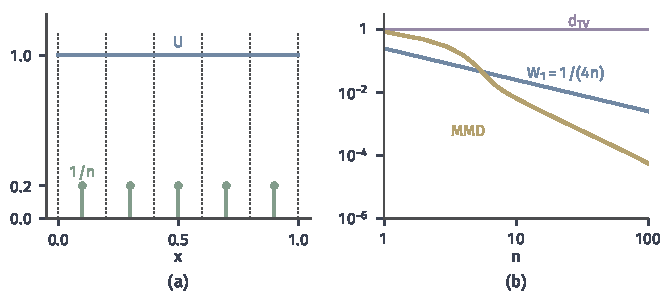
\includegraphics[width=112mm]{figures/07-probability/04-distribution-analysis/matplotlib/dcomp-lattice-metrics/figure.pdf}
 \caption{格点均匀分布逼近$\operatorname{Unif}(0,1)$。(a)$n=5$：绿色竖线是格点上的质量$1/n$，蓝线是$U$的密度，深灰点线是小区间的分界。(b)双对数坐标下的$d_{\mathrm{TV}}(U_n,U)=1$（紫），$W_1(U_n,U)=1/(4n)$（蓝），$\sigma=0.1$高斯核的$\operatorname{MMD}(U_n,U)$（黄，由式~\eqref{eq:dcomp-mmd-kernel}的三个核期望计算）。}
 \label{fig:dcomp-lattice-metrics}
\end{BookInlineFigure}

\subsection{Wasserstein收敛}
\label{sec:dcomp-wasserstein-convergence}

上一小节的格点例子中，$W_1\to0$与弱收敛同时成立。第~\ref{sec:dcomp-tail}节的$P_n=(1-\tfrac1n)\delta_0+\tfrac1n\delta_n$弱收敛到$\delta_0$（对有界连续$f$，$\int f\,\mathrm{d}P_n$与$f(0)$之差是$(f(n)-f(0))/n$，趋于零），$W_1(P_n,\delta_0)$却恒为$1$。差别在于一阶矩：$P_n$的均值恒为$1$，不收敛到$0$。下面的定理说明，这正是两者之间的全部差别。

\begin{theorem}[Wasserstein收敛的刻画]
\label{thm:dcomp-wasserstein-convergence}
设$(E,d)$是Polish空间，$1\leq p<\infty$，$\mu_n,\mu\in\mathcal{P}_p(E)$，$x_0\in E$。则$W_p(\mu_n,\mu)\to0$当且仅当
\begin{equation}
 \mu_n\xrightarrow{\mathrm{w}}\mu\quad\text{且}\quad\int d(x,x_0)^{p}\,\mu_n(\mathrm{d}x)\to\int d(x,x_0)^{p}\,\mu(\mathrm{d}x) .
 \label{eq:dcomp-wasserstein-convergence}
\end{equation}
\end{theorem}

下面证明“仅当”。“当”的方向需要从弱收敛与矩收敛出发构造代价趋于零的耦合，要用到$p$阶矩的一致可积与紧集上的逼近，篇幅较长，读者可查阅~\scite{math-villani2009transport}。

\begin{proof}[“仅当”的证明]
对每个$n$取耦合$\pi_n\in\Pi(\mu_n,\mu)$，使其成本不超过$W_p^{p}(\mu_n,\mu)+1/n$，并设随机变量对$(X_n,X)$服从$\pi_n$（每个$n$用各自的概率空间）。于是
\[
 \varepsilon_n=\bigl(\mathbb{E}\,d(X_n,X)^{p}\bigr)^{1/p}\to0 .
\]

\emph{弱收敛。}设$f$有界且Lipschitz，常数为$L$。由Lyapunov不等式$\mathbb{E}\,d(X_n,X)\leq\varepsilon_n$，
\[
 \Bigl\lvert\int f\,\mathrm{d}\mu_n-\int f\,\mathrm{d}\mu\Bigr\rvert\leq\mathbb{E}\bigl\lvert f(X_n)-f(X)\bigr\rvert\leq L\,\varepsilon_n\to0 .
\]
由Portmanteau定理的有界Lipschitz判据，$\mu_n\xrightarrow{\mathrm{w}}\mu$。

\emph{矩的收敛。}由三角不等式$d(X_n,x_0)\leq d(X_n,X)+d(X,x_0)$与$L^{p}$范数的Minkowski不等式，
\[
 \bigl(\mathbb{E}\,d(X_n,x_0)^{p}\bigr)^{1/p}\leq\varepsilon_n+\bigl(\mathbb{E}\,d(X,x_0)^{p}\bigr)^{1/p} .
\]
交换$X_n$与$X$的角色得到反向不等式，所以两个$p$阶矩的$p$次根之差不超过$\varepsilon_n$，趋于零。
\end{proof}

定理给出了一个清楚的分工：弱收敛管住质量在有界范围内的摆放，矩收敛管住远处有多少质量。第~\ref{sec:dcomp-tail}节的$R_n=(1-n^{-2})\delta_0+n^{-2}\delta_n$是一个检验：它弱收敛到$\delta_0$，一阶矩$1/n\to0$，二阶矩恒为$1$，所以$W_1\to0$而$W_2\not\to0$，与图~\ref{fig:dcomp-far-mass}(b)一致。阶数$p$越高，对远处质量的要求越严。

\paragraph{分布收敛不是取值收敛}
$W_p(\mu_n,\mu)\to0$说的是存在代价越来越小的耦合，而不是某个已经给定的联合实现中的误差变小。设$X\sim\mathcal{N}(0,1)$，$X'$是它的独立副本。$X'$与$X$同分布，$W_p(P_{X'},P_X)=0$，最优耦合是让两者相等。可是在已经给定的独立实现中，
\[
 \mathbb{E}\bigl[(X'-X)^{2}\bigr]=\operatorname{Var}(X')+\operatorname{Var}(X)=2 .
\]
把$X'$换成序列$X_n=X'$（每个$n$都相同），就有$W_2(P_{X_n},P_X)=0$对一切$n$成立，而$\mathbb{E}\lvert X_n-X\rvert^{2}=2$不趋于零。图~\ref{fig:dcomp-coupling-realization}用$300$个模拟点（种子$717$）对比这两种耦合，独立实现的样本平均平方差约为$1.94$。Wasserstein距离只是一个关于分布的结论，不能反推原有共同实现中的$L^{p}$误差；后者是第~\ref{chap:random-variable-convergence}章的$L^{p}$收敛，它要求$X_n$与$X$在同一概率空间上逐点接近。

\begin{BookInlineFigure}
 \centering
 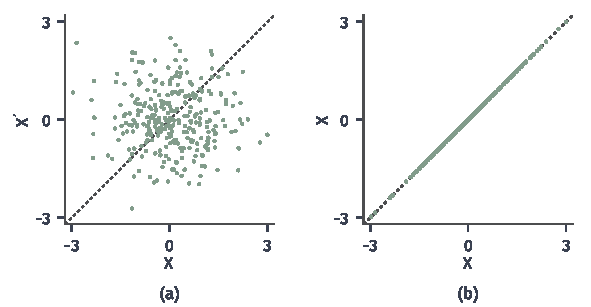
\includegraphics[width=100mm]{figures/07-probability/04-distribution-analysis/matplotlib/dcomp-coupling-realization/figure.pdf}
 \caption{$\mathcal{N}(0,1)$与自身的两种耦合，各$300$个模拟点（绿），种子$717$；深灰点线是$y=x$。(a)独立副本$(X,X')$，$\mathbb{E}(X-X')^{2}=2$，样本值约$1.94$。(b)恒等耦合$(X,X)$，成本为$0=W_2^{2}$。}
 \label{fig:dcomp-coupling-realization}
\end{BookInlineFigure}

\subsection{MMD收敛}
\label{sec:dcomp-mmd-convergence}

特征核保证$\operatorname{MMD}_k(P,Q)=0$当且仅当$P=Q$。一列分布的MMD趋于零是否等价于弱收敛，是另一回事：零点的辨识只涉及单个分布对，收敛还要求比较量不让质量悄悄跑到无穷远，也不对微小平移过度敏感。对$\mathbb{R}^{d}$上固定带宽的高斯核，两件事都成立。

\begin{theorem}[高斯核MMD刻画弱收敛]
\label{thm:dcomp-mmd-weak}
设$\sigma>0$，$k_\sigma$是$\mathbb{R}^{d}$上的高斯核，$P_n,P$是$\mathbb{R}^{d}$上的概率分布。则
\begin{equation}
 \operatorname{MMD}_{k_\sigma}(P_n,P)\to0\quad\Longleftrightarrow\quad P_n\xrightarrow{\mathrm{w}}P .
 \label{eq:dcomp-mmd-weak}
\end{equation}
\end{theorem}

\begin{proof}
\emph{弱收敛推出MMD趋于零。}取相互独立的$\bm{X}_n,\bm{X}_n'\sim P_n$与$\bm{X},\bm{X}'\sim P$。由第~\ref{chap:weak-convergence-of-distributions}章独立分量的联合极限，$(\bm{X}_n,\bm{X}_n')$与$(\bm{X}_n,\bm{X})$都依分布收敛到$(\bm{X},\bm{X}')$。$k_\sigma$在$\mathbb{R}^{d}\times\mathbb{R}^{d}$上有界连续，所以式~\eqref{eq:dcomp-mmd-kernel}中的三项分别趋于$\mathbb{E}[k_\sigma(\bm{X},\bm{X}')]$的$1$倍、$2$倍与$1$倍，和趋于零。

\emph{MMD趋于零推出胎紧。}记$\phi_n,\phi$为特征函数，$\lambda_\sigma$与$\gamma_\tau$分别为$\mathcal{N}(\bm{0},\sigma^{-2}\bm{I})$与$\mathcal{N}(\bm{0},\tau\bm{I})$的密度。令
\[
 h_\tau(\bm{x})=\exp\Bigl(-\frac{\tau}{2}\lVert\bm{x}\rVert_2^{2}\Bigr) .
\]
它是$\mathcal{N}(\bm{0},\tau\bm{I})$的特征函数，由Fubini定理，
\[
 \mathbb{E}_{P_n}[h_\tau]=\int\phi_n(\bm{\omega})\,\gamma_\tau(\bm{\omega})\,\mathrm{d}\bm{\omega} .
\]
于是，由Cauchy--Schwarz不等式与式~\eqref{eq:dcomp-mmd-spectral}，
\[
 \begin{aligned}
 \bigl\lvert\mathbb{E}_{P_n}[h_\tau]-\mathbb{E}_{P}[h_\tau]\bigr\rvert&\leq\int\lvert\phi_n-\phi\rvert\frac{\gamma_\tau}{\lambda_\sigma}\lambda_\sigma\,\mathrm{d}\bm{\omega}\\
 &\leq\operatorname{MMD}_{k_\sigma}(P_n,P)\Bigl(\int\frac{\gamma_\tau^{2}}{\lambda_\sigma}\,\mathrm{d}\bm{\omega}\Bigr)^{1/2} .
 \end{aligned}
\]
$\gamma_\tau^{2}/\lambda_\sigma$正比于$\exp(-(\tau^{-1}-\sigma^{2}/2)\lVert\bm{\omega}\rVert_2^{2})$，当$\tau<2/\sigma^{2}$时可积。所以对这样的$\tau$，$\mathbb{E}_{P_n}[h_\tau]\to\mathbb{E}_{P}[h_\tau]$。

任给$\varepsilon>0$。$\tau\downarrow0$时$h_\tau\uparrow1$，由单调收敛定理可取$\tau<2/\sigma^{2}$使$1-\mathbb{E}_{P}[h_\tau]<\varepsilon$，再取$N$使$n\geq N$时$1-\mathbb{E}_{P_n}[h_\tau]<2\varepsilon$。取$r$使$\mathrm{e}^{-\tau r^{2}/2}\leq\tfrac12$。在$\{\lVert\bm{x}\rVert_2>r\}$上$1-h_\tau\geq\tfrac12$，由Markov不等式，
\[
 P_n\bigl(\lVert\bm{X}\rVert_2>r\bigr)\leq2\bigl(1-\mathbb{E}_{P_n}[h_\tau]\bigr)<4\varepsilon,\qquad n\geq N .
\]
前$N-1$个分布各自胎紧，增大$r$即可一并照顾，所以$\{P_n\}$胎紧。

\emph{子列的极限只能是$P$。}设某个子列$P_{n_j}\xrightarrow{\mathrm{w}}R$。由连续性定理，$\phi_{n_j}\to\phi_R$逐点成立，并且都以$1$为界，由控制收敛定理，$\phi_{n_j}$在$L^{2}(\Lambda_\sigma)$中收敛到$\phi_R$。又由式~\eqref{eq:dcomp-mmd-spectral}，$\phi_{n_j}$在$L^{2}(\Lambda_\sigma)$中到$\phi$的距离就是MMD，趋于零。由$L^{2}(\Lambda_\sigma)$中的三角不等式，$\phi_R=\phi$在$\Lambda_\sigma$几乎处处成立。与定理~\ref{thm:dcomp-gauss-characteristic}的论证相同，$R=P$。由第~\ref{chap:weak-convergence-of-distributions}章的子列原则，$P_n\xrightarrow{\mathrm{w}}P$。
\end{proof}

证明里高斯核起了两个作用。谱权重$\Lambda_\sigma$处处为正，保证极限唯一；它的尾部比$\gamma_\tau^{2}$的尾部衰减得慢，使原点附近的特征函数，也就是“质量是否跑远”的信息，能被MMD控制住。

\paragraph{结论的边界}
高斯核MMD刻画的是弱收敛，不多也不少。它不附带矩的收敛：$P_n=(1-\tfrac1n)\delta_0+\tfrac1n\delta_n$弱收敛到$\delta_0$，所以MMD趋于零（图~\ref{fig:dcomp-far-mass}(a)），均值却恒为$1$。要控制无界函数，仍需第~\ref{sec:dcomp-tail}节的尾部条件。

这个刻画也不能推广到所有特征核。在高斯核上加一个不连续的部分：令$f=\mathbf{1}_{(0,\infty)}$，
\[
 k(x,y)=k_1(x,y)+f(x)f(y),\qquad x,y\in\mathbb{R} .
\]
两个正定核之和仍是正定核，它有界，可以验证相应的RKHS可分、特征映射可测。由式~\eqref{eq:dcomp-mmd-kernel}，
\[
 \operatorname{MMD}_k^{2}(P,Q)=\operatorname{MMD}_{k_1}^{2}(P,Q)+\bigl(P(X>0)-Q(X>0)\bigr)^{2}\geq\operatorname{MMD}_{k_1}^{2}(P,Q),
\]
所以$k$仍是特征核。可是$\delta_{1/n}\xrightarrow{\mathrm{w}}\delta_0$，而第二项恒为$(1-0)^{2}=1$，$\operatorname{MMD}_k(\delta_{1/n},\delta_0)\geq1$不趋于零。不连续的核截面像示性函数一样对微小平移敏感。所以“MMD收敛等价于弱收敛”须同时核对空间与核的条件，例如核的连续性与有界性，不能只凭特征性得出。

\section{本章小结}
\label{sec:dcomp-summary}

章首的问题是：两份概率表$P=(0.6,0.3,0.1)$与$Q=(0.3,0.3,0.4)$差多少。本章的回答是，先问差别会在哪里造成后果，再选比较量。表~\ref{tab:dcomp-summary-example}把例表上算出的各个量放在一起。

\begin{BookInlineTable}
 \centering
 \caption{例表上的各比较量（自然对数；MMD用$\sigma=1$的高斯核）。}
 \label{tab:dcomp-summary-example}
 \begin{tabular}{lll}
  \toprule
  比较量 & 数值 & 回答的问题\\
  \midrule
  $d_{\mathrm{TV}}$ & $0.3$ & 同一事件的概率最多差多少\\
  $D_{\mathrm{KL}}(P\Vert Q)$，$D_{\mathrm{KL}}(Q\Vert P)$ & $0.2773$，$0.3466$ & 平均对数比，方向不同\\
  $d_{\mathrm{H}}$，$B$ & $0.2752$，$0.9243$ & 平方根密度的弦长与重叠\\
  $D_{\mathrm{JS}}$ & $0.0737$ & 相对平均分布的KL，有界\\
  $D_{1/2}$，$D_{2}$ & $0.1575$，$0.4220$ & 不同幂次加权的对数比\\
  $\operatorname{MMD}_k$ & $0.3945$ & 核均值之差\\
  $W_1$，$W_2$ & $0.6$，$0.7746$ & 搬运质量的最小成本\\
  \bottomrule
 \end{tabular}
\end{BookInlineTable}

四个角度各有所长。总变差控制所有事件与有界函数，不需要底层距离，但对微小平移与相互奇异的分布一律给出最大值。密度比较量在同一支配测度下比较同一位置的权重：KL散度有似然比的含义并且不对称，Hellinger距离是平方根密度之间的真正距离，JS散度借助平均分布保持有限，Rényi散度用阶数调节对大比值的敏感程度；它们中的$f$散度都满足后处理不增的性质。积分概率度量由测试函数类决定能看见什么，核均值把RKHS单位球上的上确界变成两个核均值之差的范数。Wasserstein距离保留底层几何，一阶时又是Lipschitz函数上的积分概率度量。

用于控制期望时，要先判断评价函数$g$的类型：有界函数配总变差，Lipschitz函数配$W_1$，RKHS中的函数配MMD；无界函数必须把尾部单独拿出来，用一致可积或高阶矩控制；用KL散度控制期望时，需要参考分布下的指数矩，并且方向要与散度的参数对应。

用于收敛时，各比较量之间的关系汇总在图~\ref{fig:dcomp-implication-map}中。KL散度通过Pinsker不等式控制总变差，总变差与Hellinger距离相互控制，总变差收敛推出弱收敛而反之不然；$W_p$收敛等于弱收敛加$p$阶矩收敛；$\mathbb{R}^{d}$上固定带宽的高斯核MMD收敛恰好等于弱收敛。反过来的每一个缺口都有反例：零概率格点使小总变差对应无穷KL，单点平移与格点逼近使弱收敛不带来总变差收敛，远处的小质量使弱收敛与MMD收敛不带来矩的收敛，不连续的特征核使MMD不再刻画弱收敛。

\begin{BookInlineFigure}
 \centering
 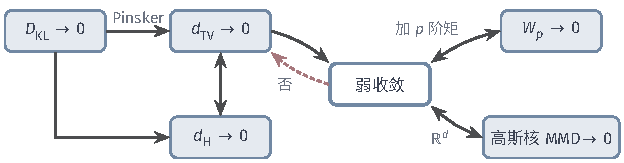
\includegraphics[width=106mm]{figures/07-probability/04-distribution-analysis/tikz/dcomp-implication-map/figure.pdf}
 \caption{本章证明或引用的收敛关系，均指$P_n$与固定的$P$之间的比较量趋于零。实线箭头表示蕴含，双向箭头表示等价（$W_p$需加上$p$阶矩收敛，高斯核MMD限于$\mathbb{R}^{d}$），红色虚线表示反向不成立。}
 \label{fig:dcomp-implication-map}
\end{BookInlineFigure}

第~\ref{chap:distribution-approximation}章在限定的候选族中寻找与目标最接近的分布时，就要用这里的比较量衡量误差，并按任务选择方向。第~\ref{chap:dependence-measures}章把联合分布与边缘乘积作比较，用KL散度得到互信息，用MMD得到HSIC。从有限样本估计这些比较量、评价估计误差并据此检验两个分布是否相同，属于卷八的内容。

